\section{Some Python Results}

\begin{figure}
%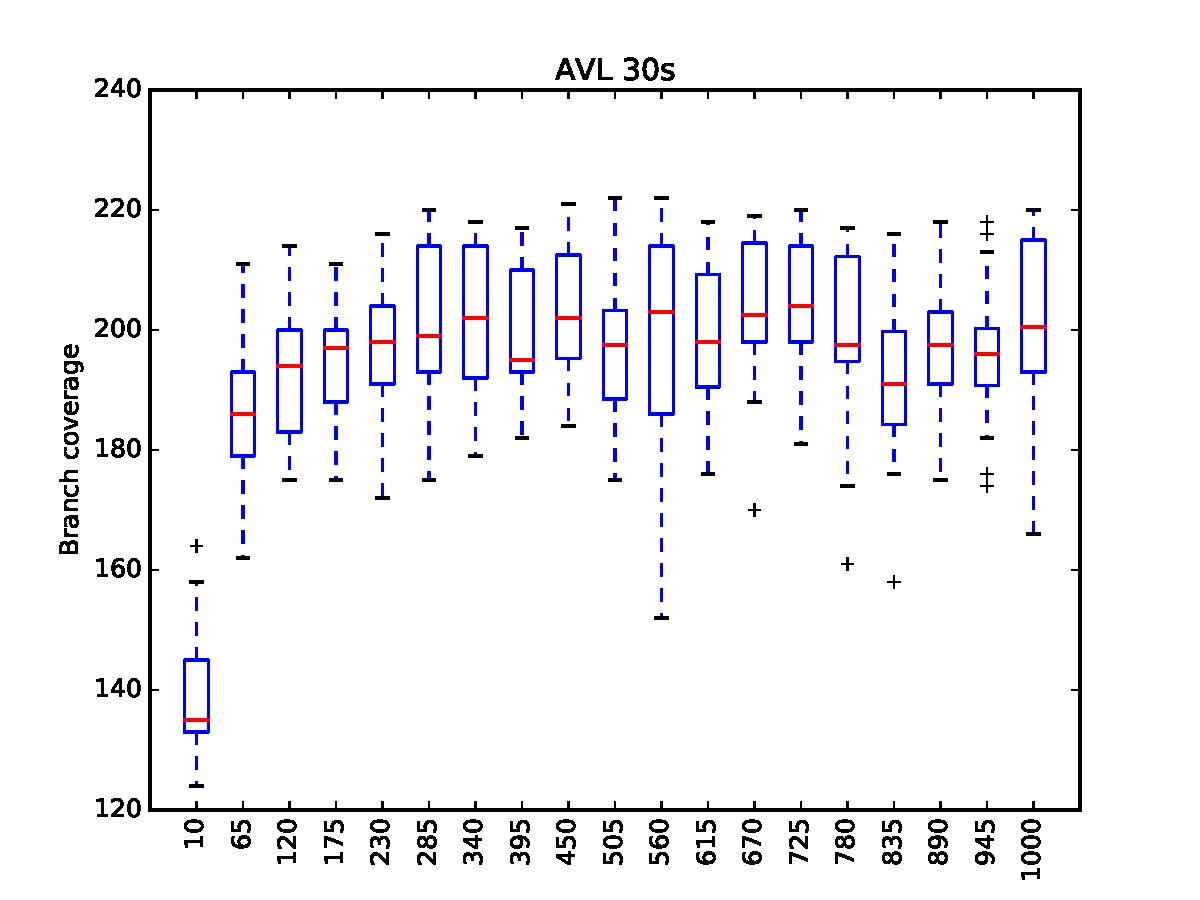
\includegraphics[width=\columnwidth]{graphs/AVLrand30}
%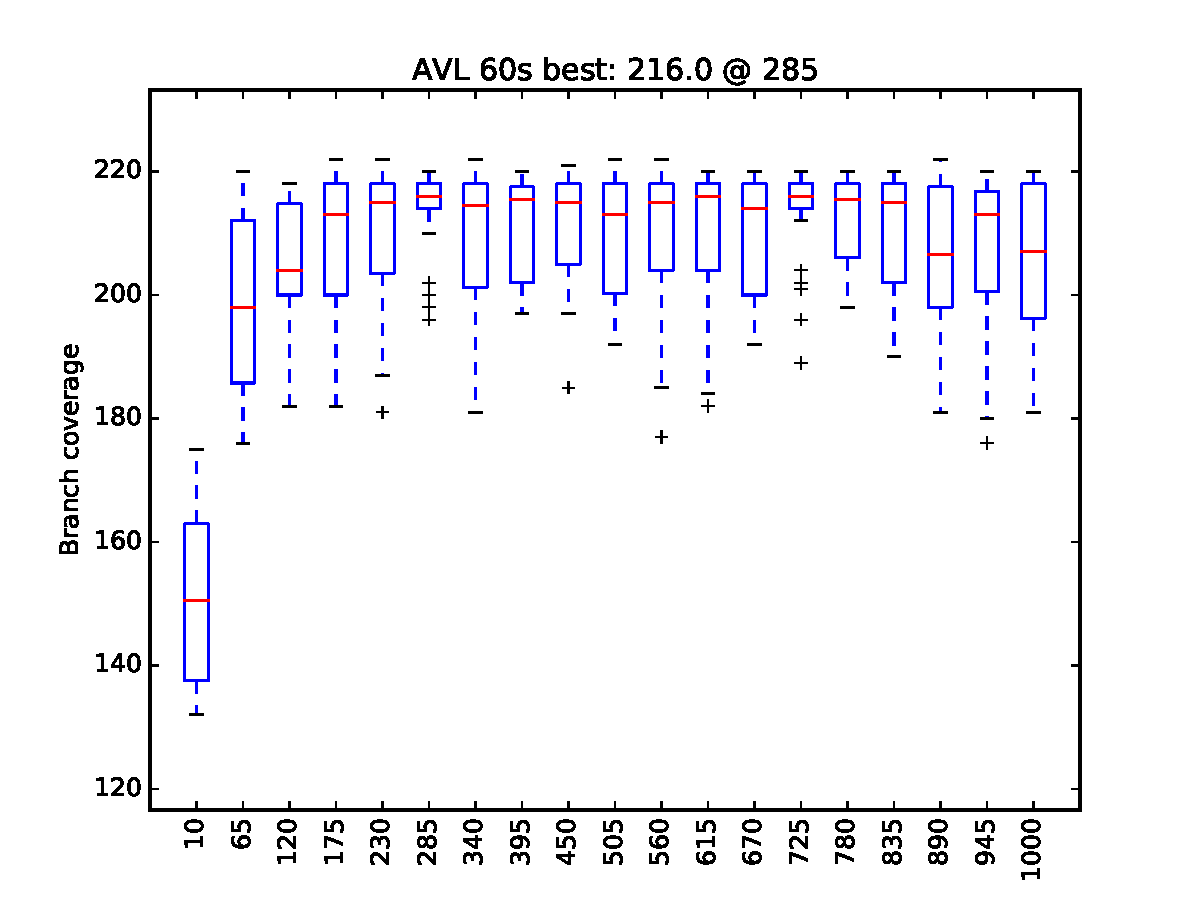
\includegraphics[width=\columnwidth]{graphs/AVLrand60}
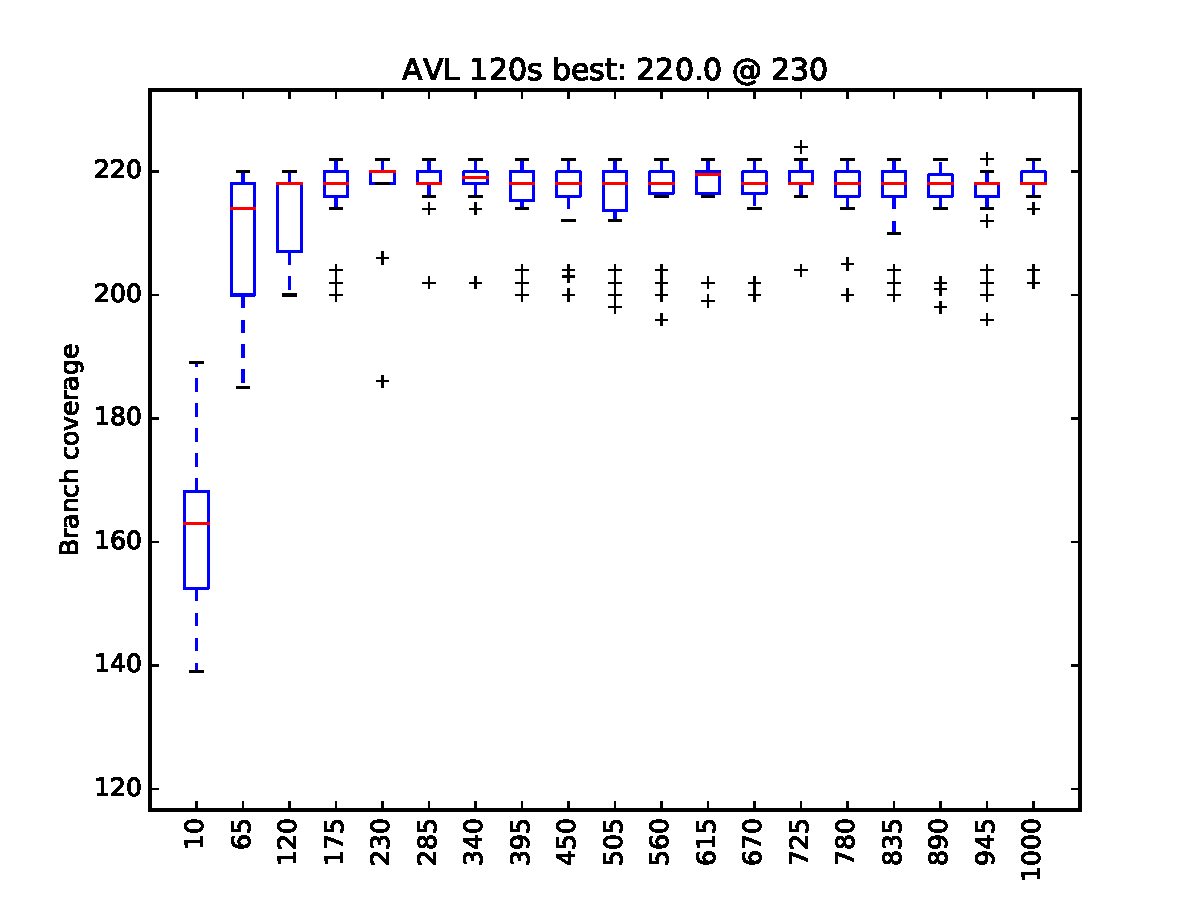
\includegraphics[width=\columnwidth]{graphs/AVLrand120}
\includegraphics[width=\columnwidth]{graphs/opsavlrand120}
\includegraphics[width=\columnwidth]{graphs/execavlrand120}
\end{figure}

\begin{figure}
%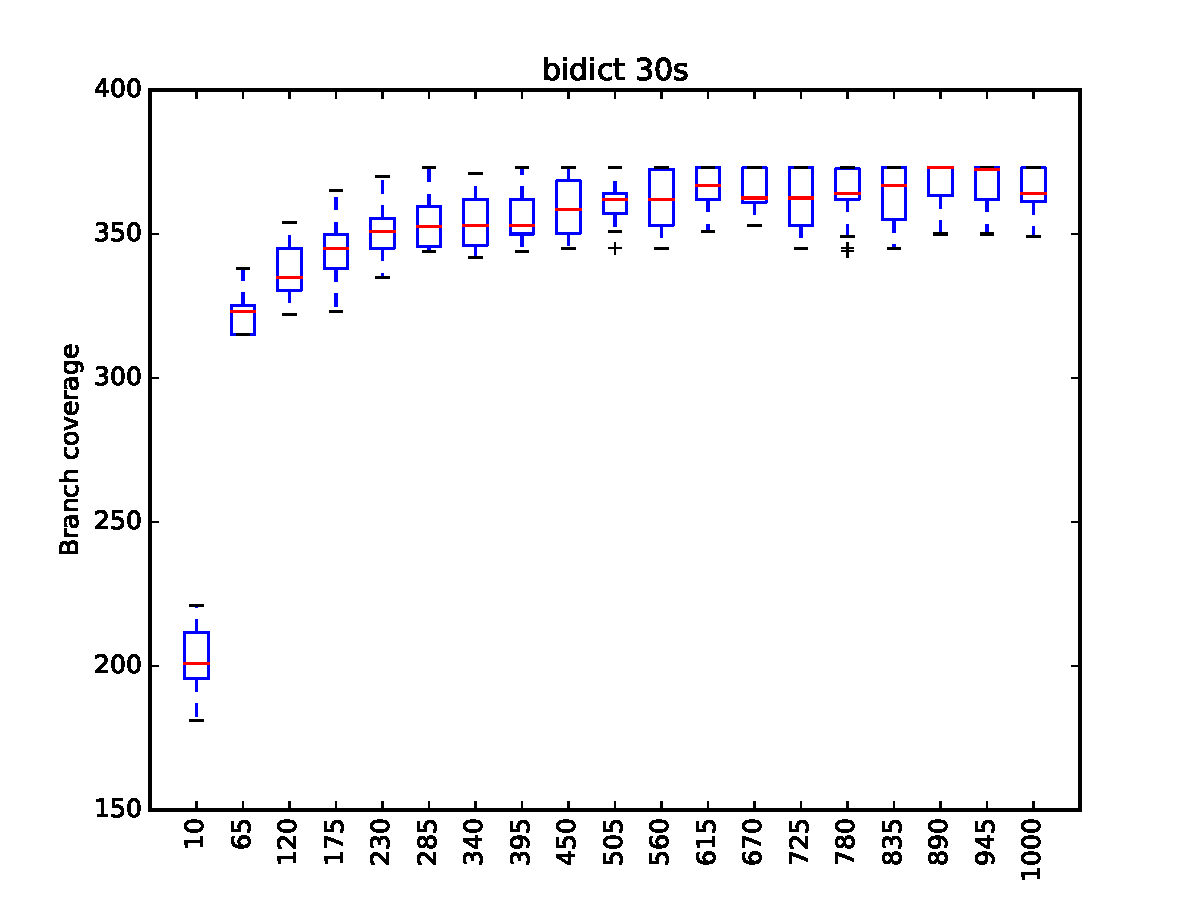
\includegraphics[width=\columnwidth]{graphs/bidictrand30}
%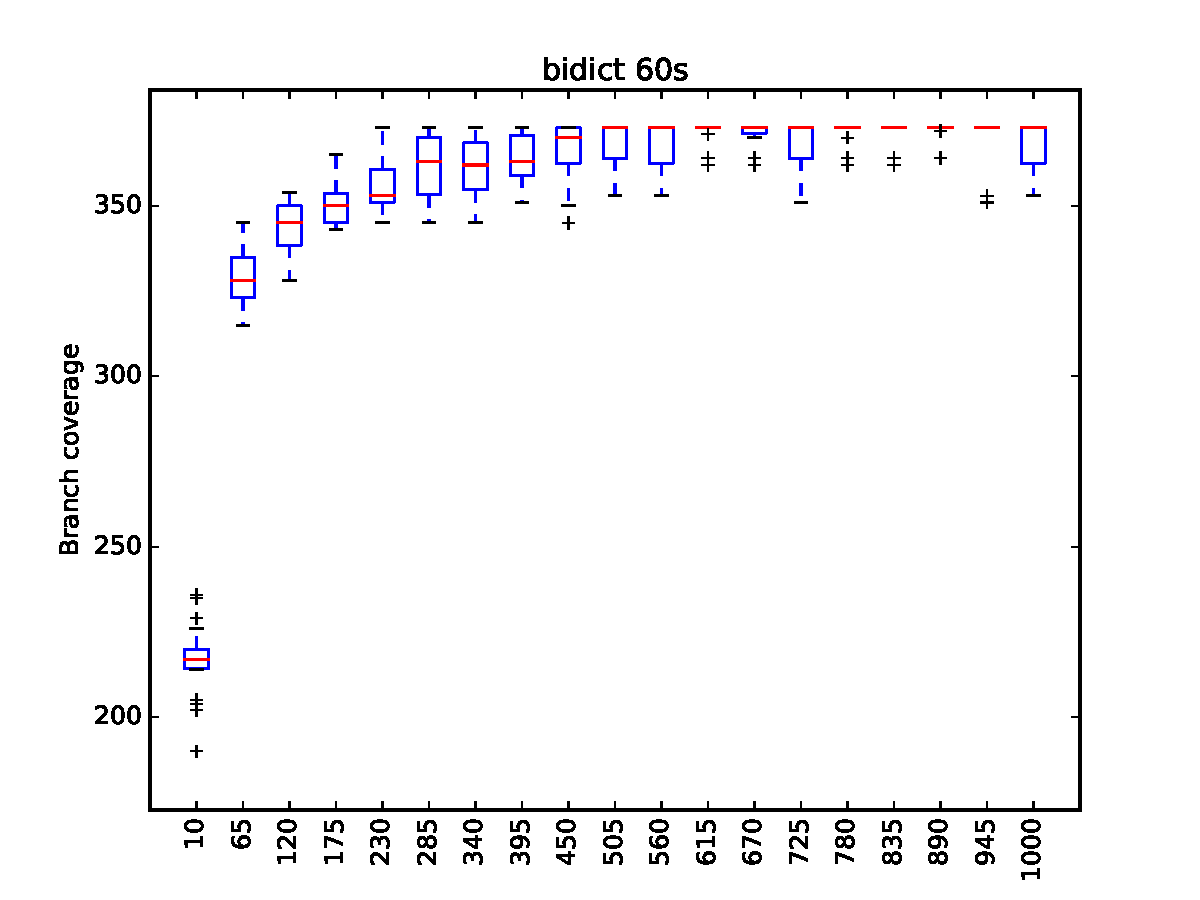
\includegraphics[width=\columnwidth]{graphs/bidictrand60}
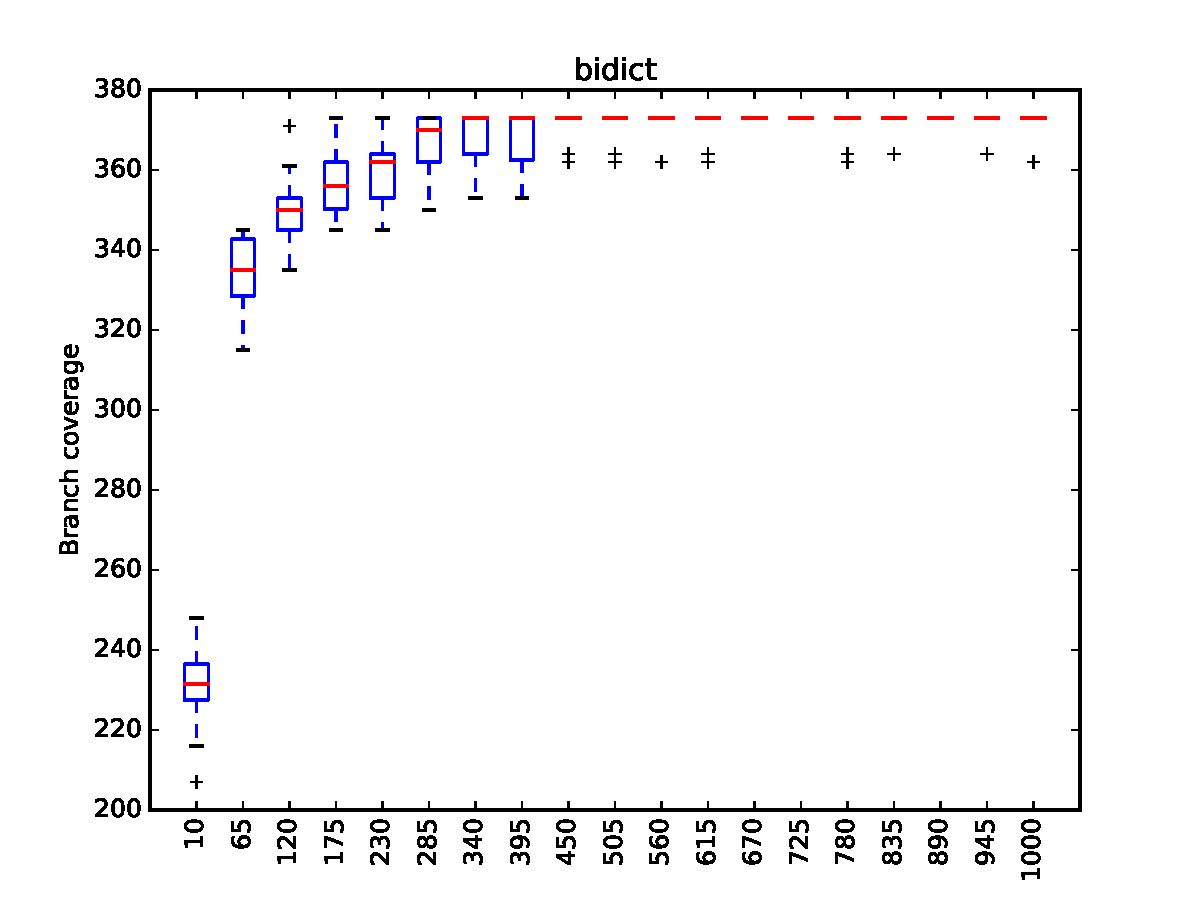
\includegraphics[width=\columnwidth]{graphs/bidictrand120}
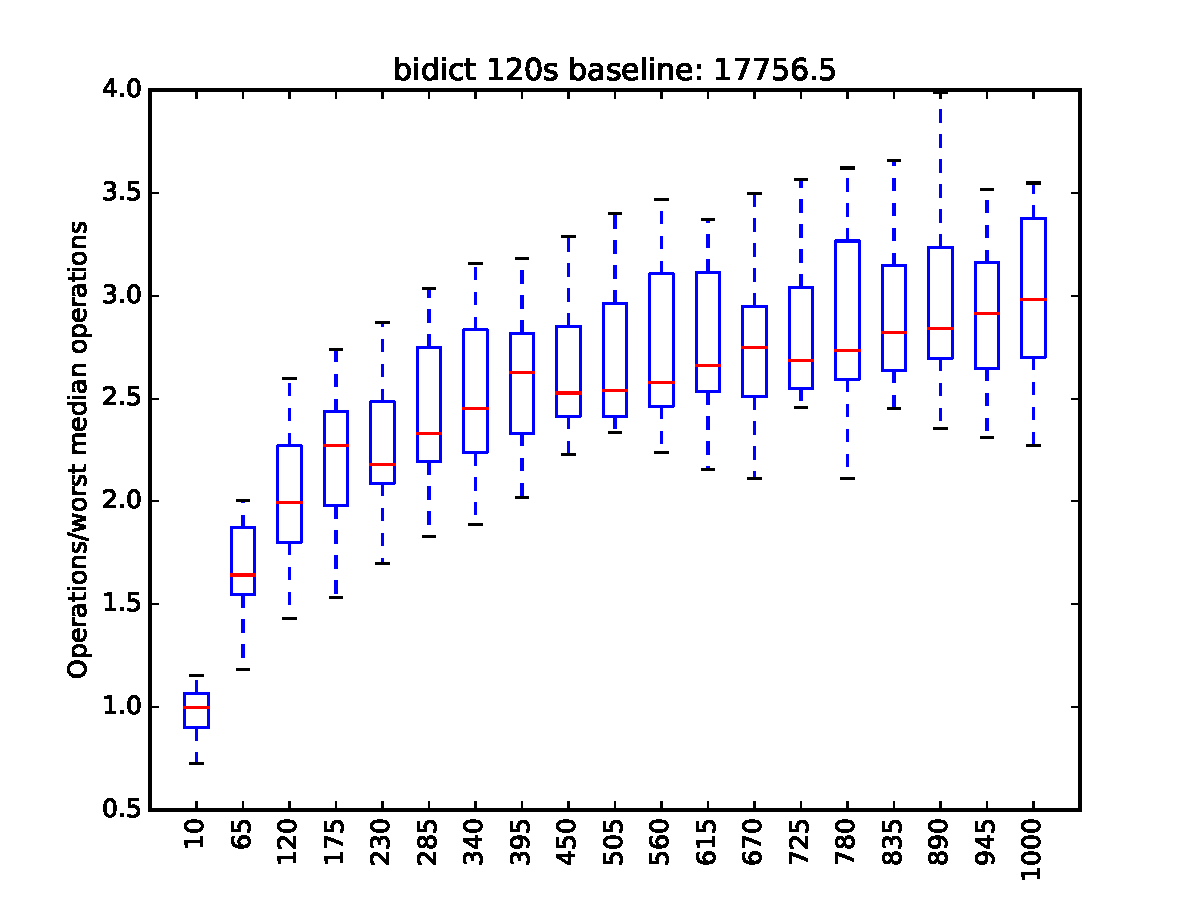
\includegraphics[width=\columnwidth]{graphs/opsbidictrand120}
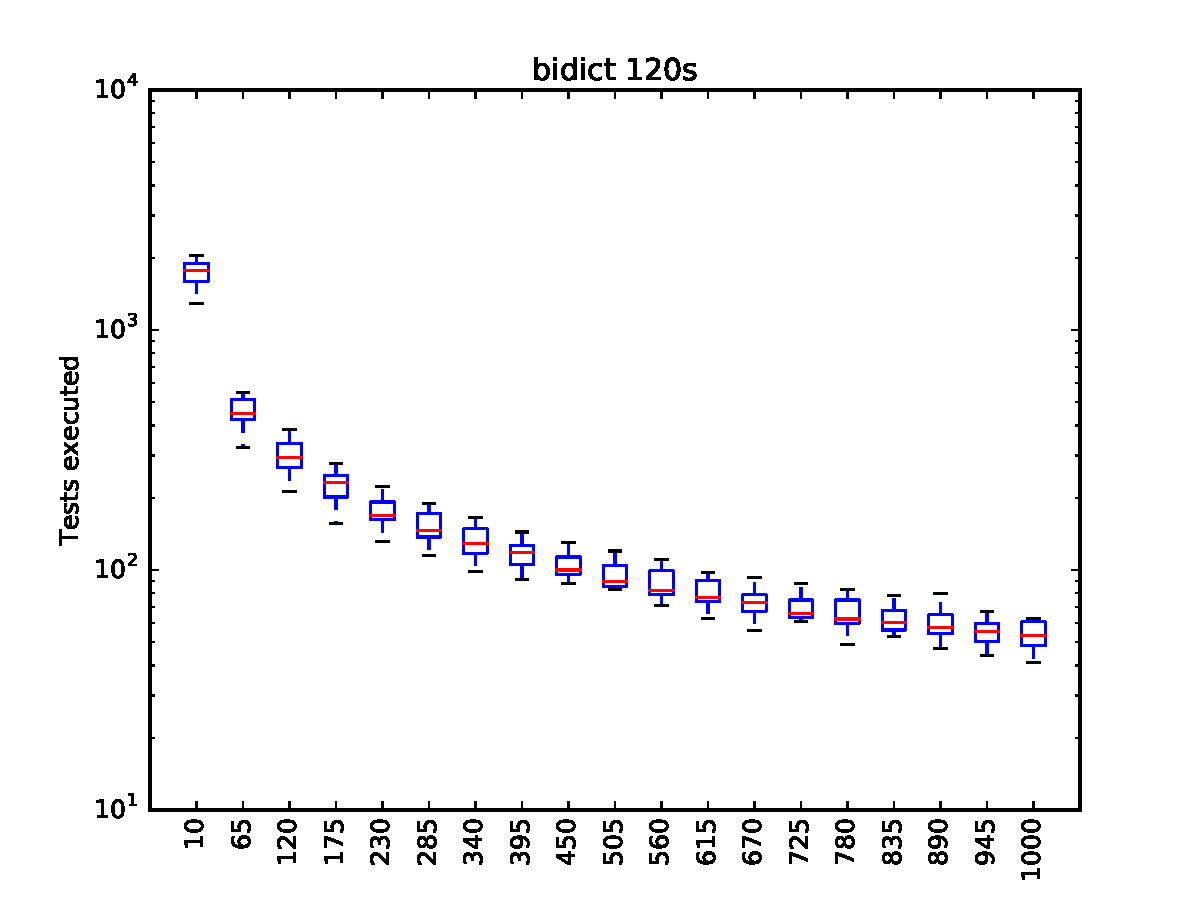
\includegraphics[width=\columnwidth]{graphs/execbidictrand120}
\end{figure}


\begin{figure}
%\includegraphics[width=\columnwidth]{graphs/Crand30}
%\includegraphics[width=\columnwidth]{graphs/Crand60}
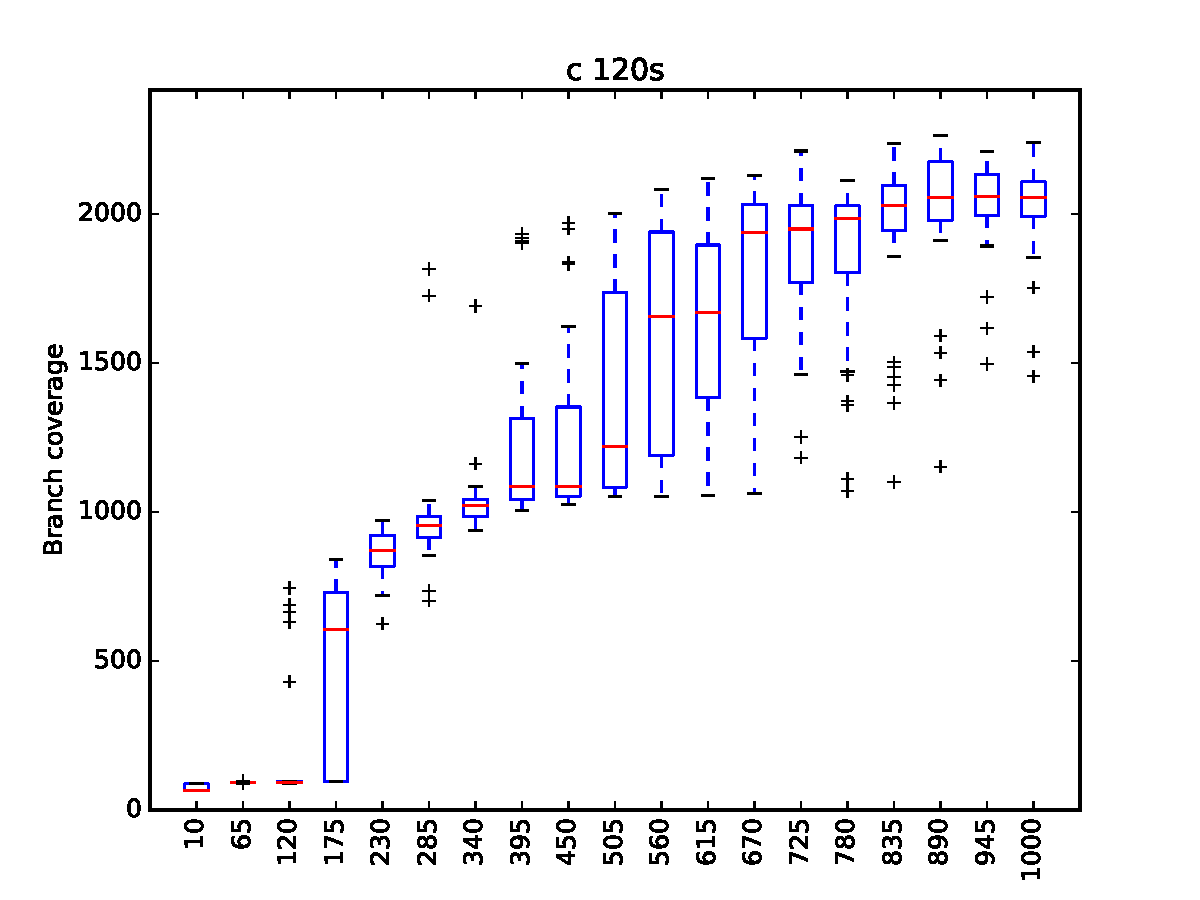
\includegraphics[width=\columnwidth]{graphs/Crand120}
\includegraphics[width=\columnwidth]{graphs/opsCrand120}
\includegraphics[width=\columnwidth]{graphs/execCrand120}
\end{figure}


\begin{figure}
%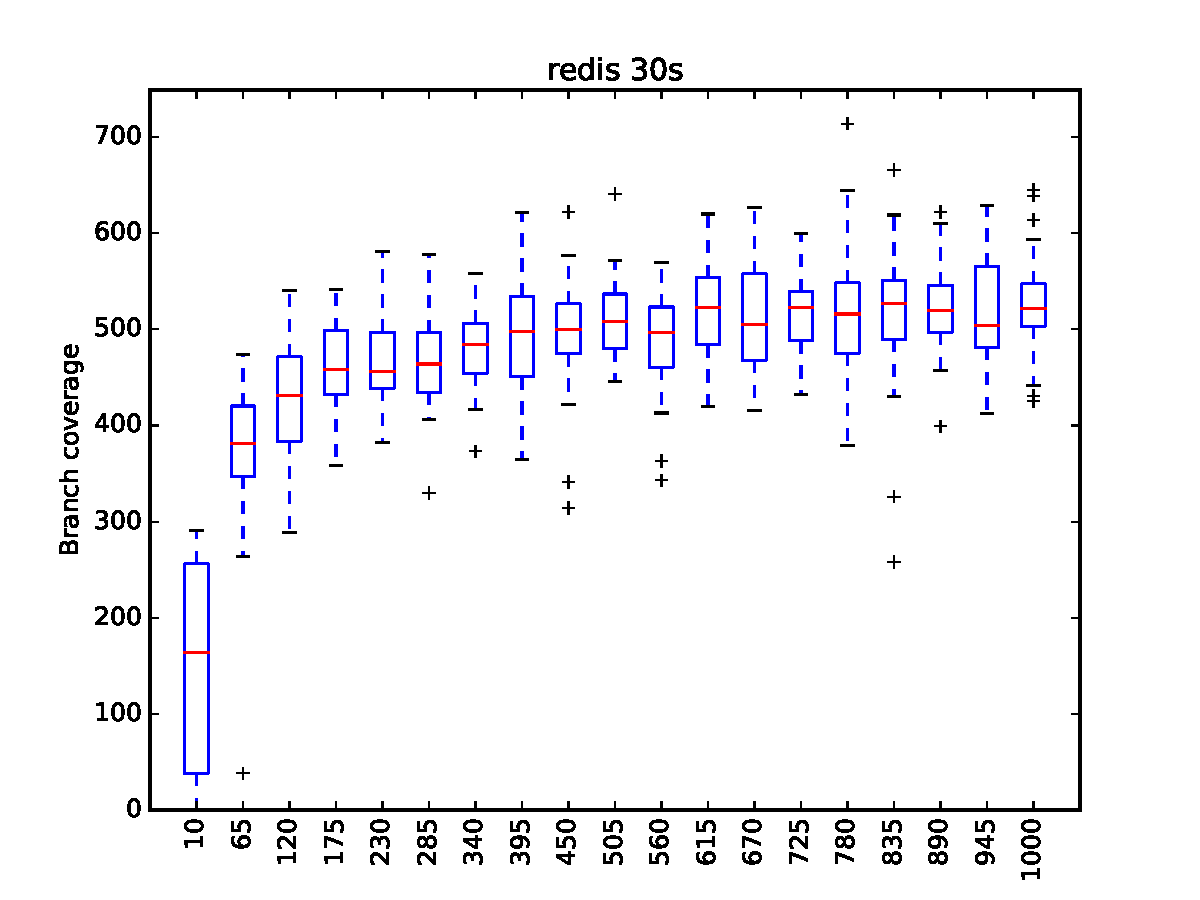
\includegraphics[width=\columnwidth]{graphs/redisrand30}
%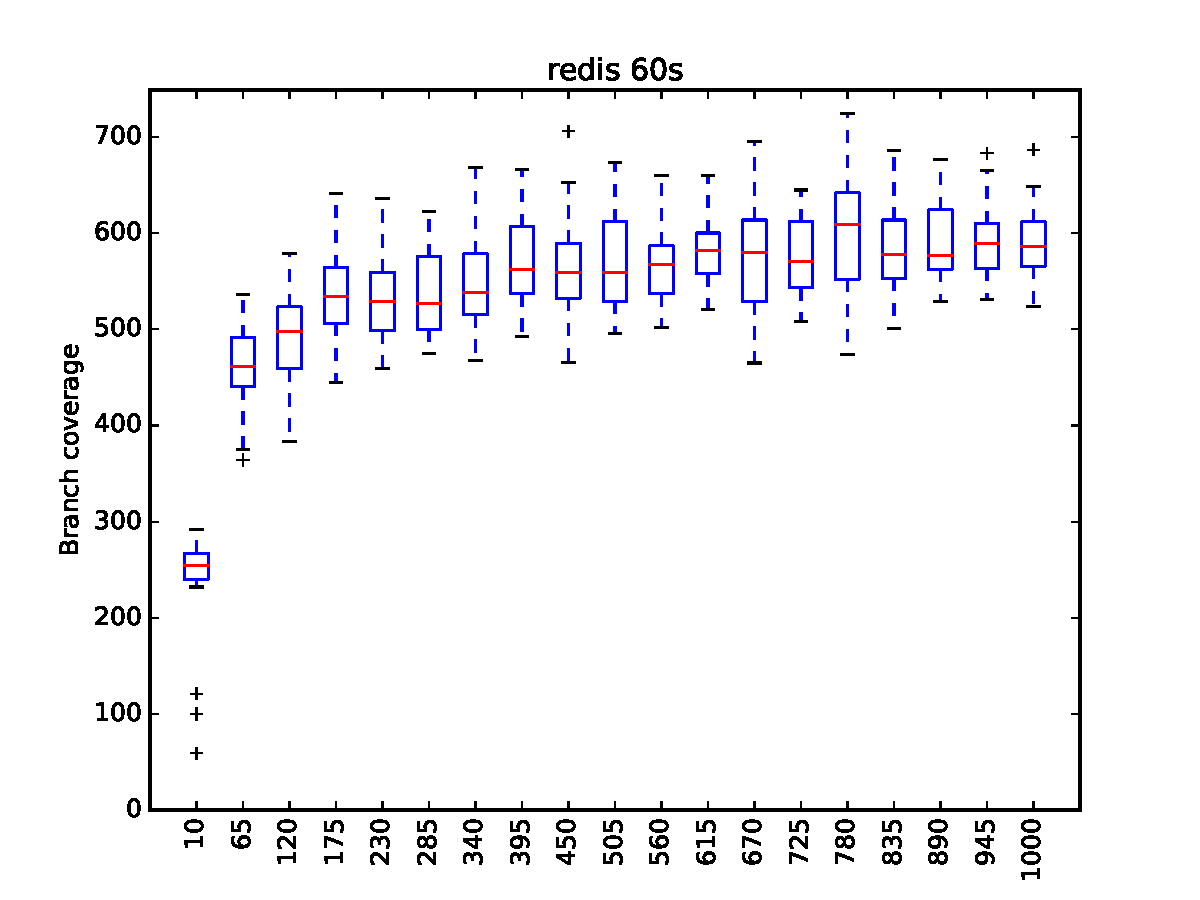
\includegraphics[width=\columnwidth]{graphs/redisrand60}
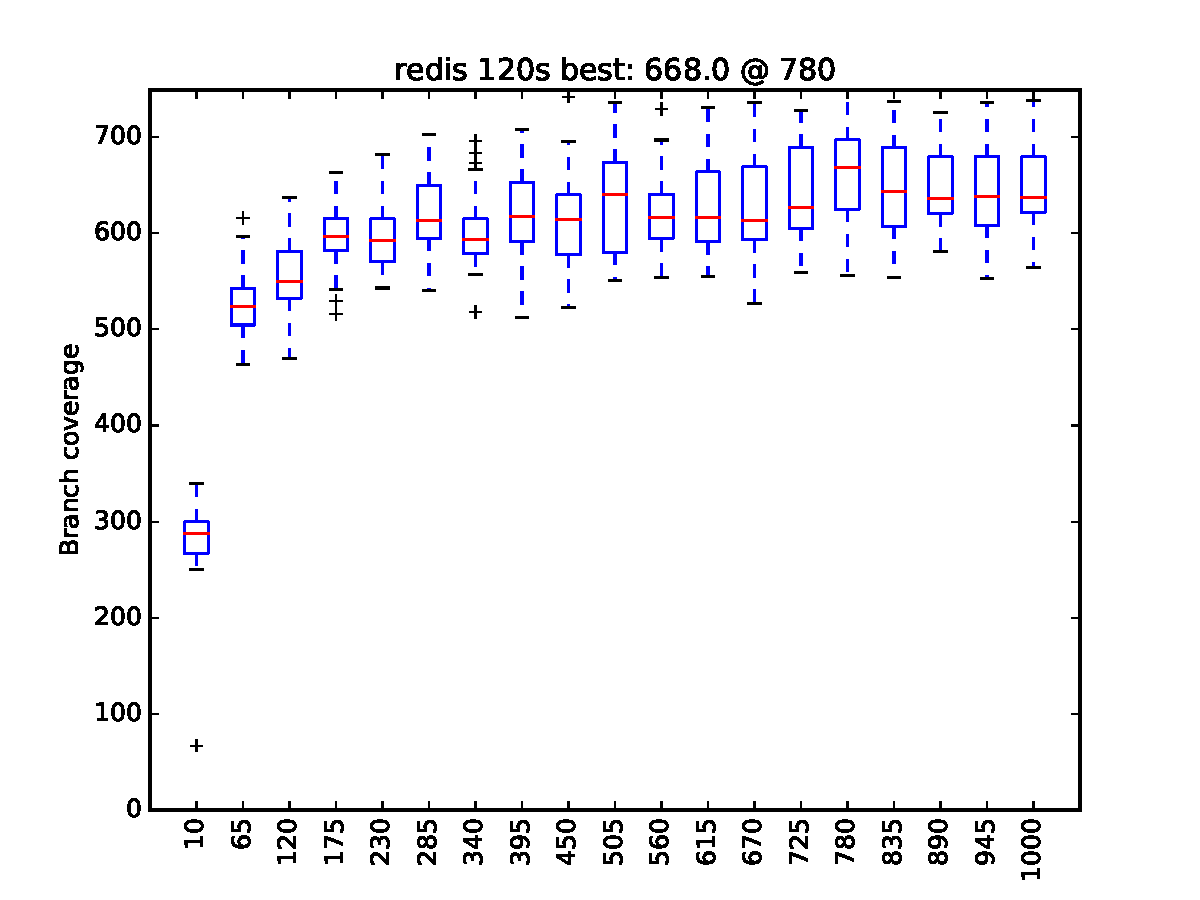
\includegraphics[width=\columnwidth]{graphs/redisrand120}
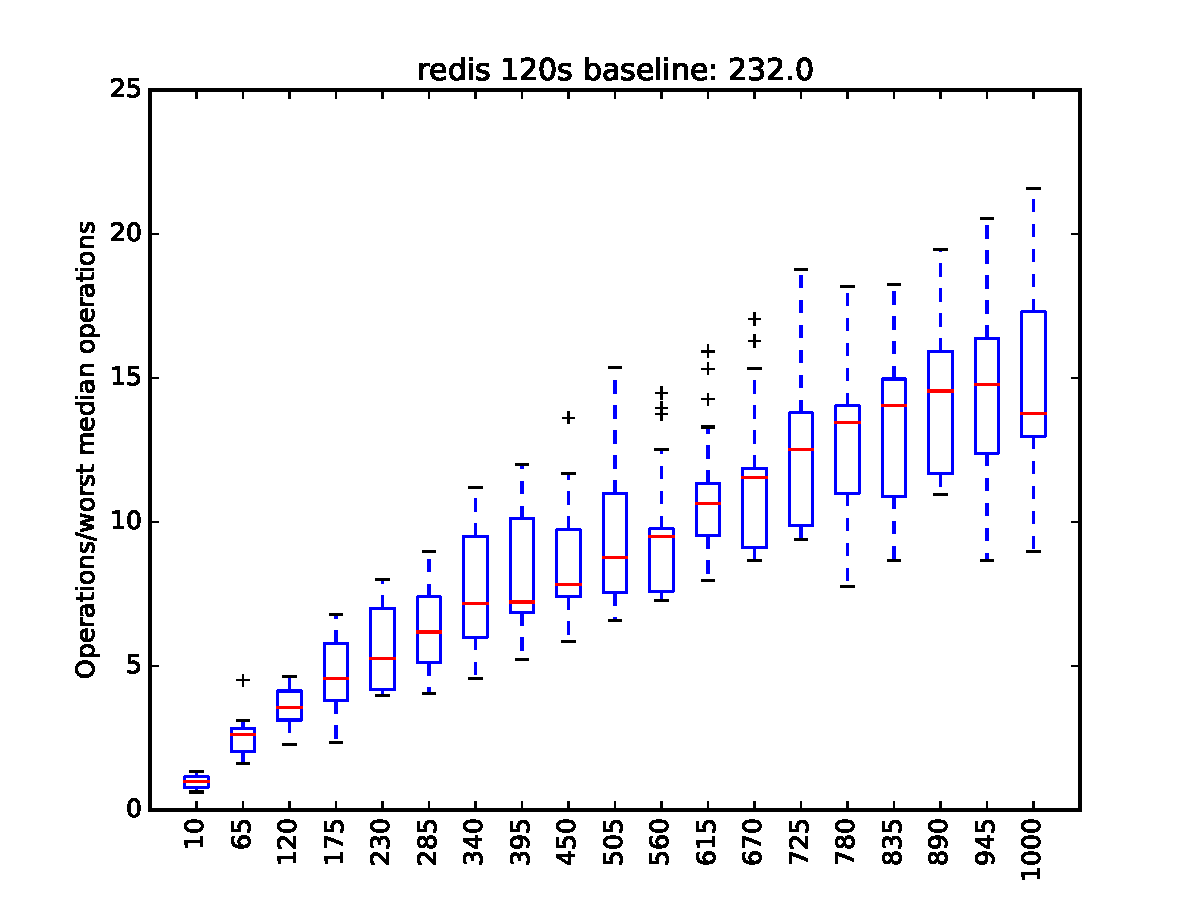
\includegraphics[width=\columnwidth]{graphs/opsredisrand120}
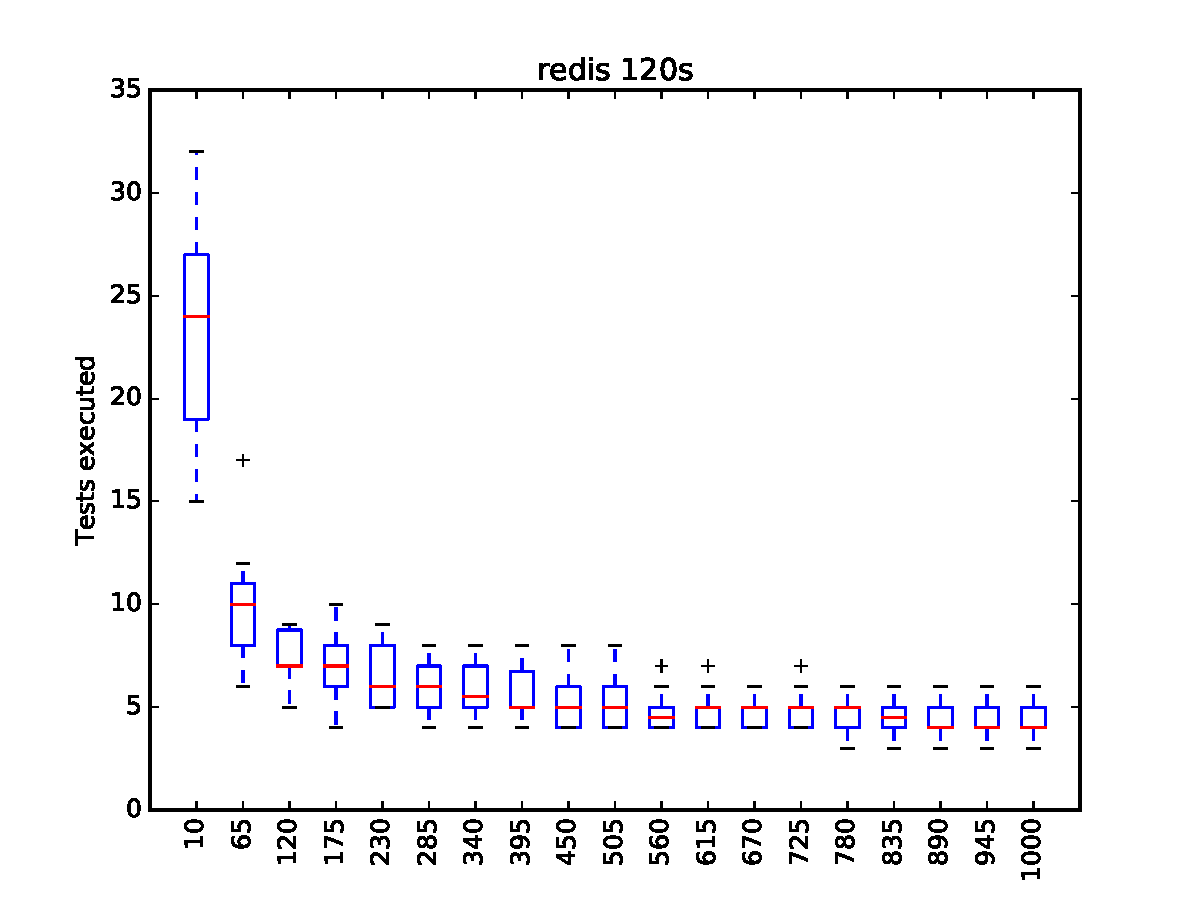
\includegraphics[width=\columnwidth]{graphs/execredisrand120}
\end{figure}

\begin{figure}
%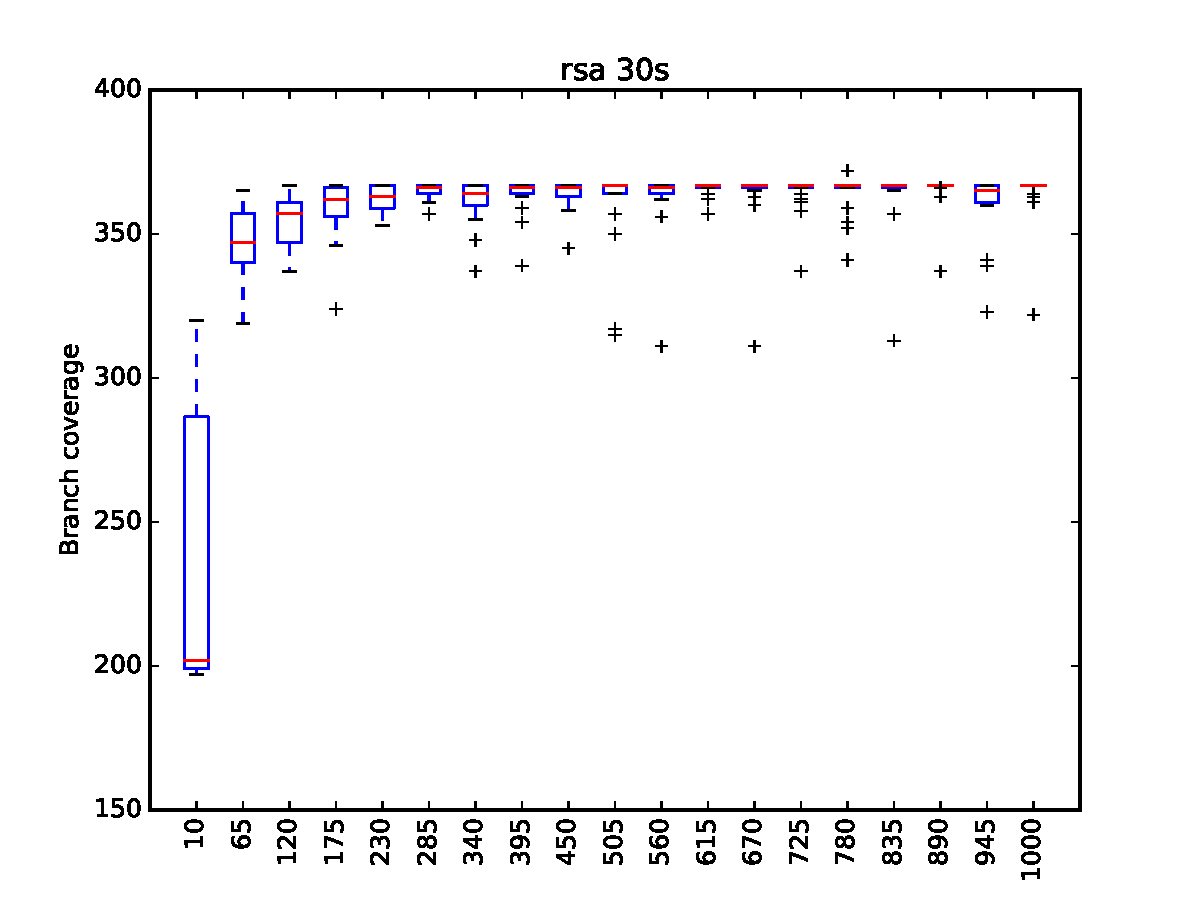
\includegraphics[width=\columnwidth]{graphs/rsarand30}
%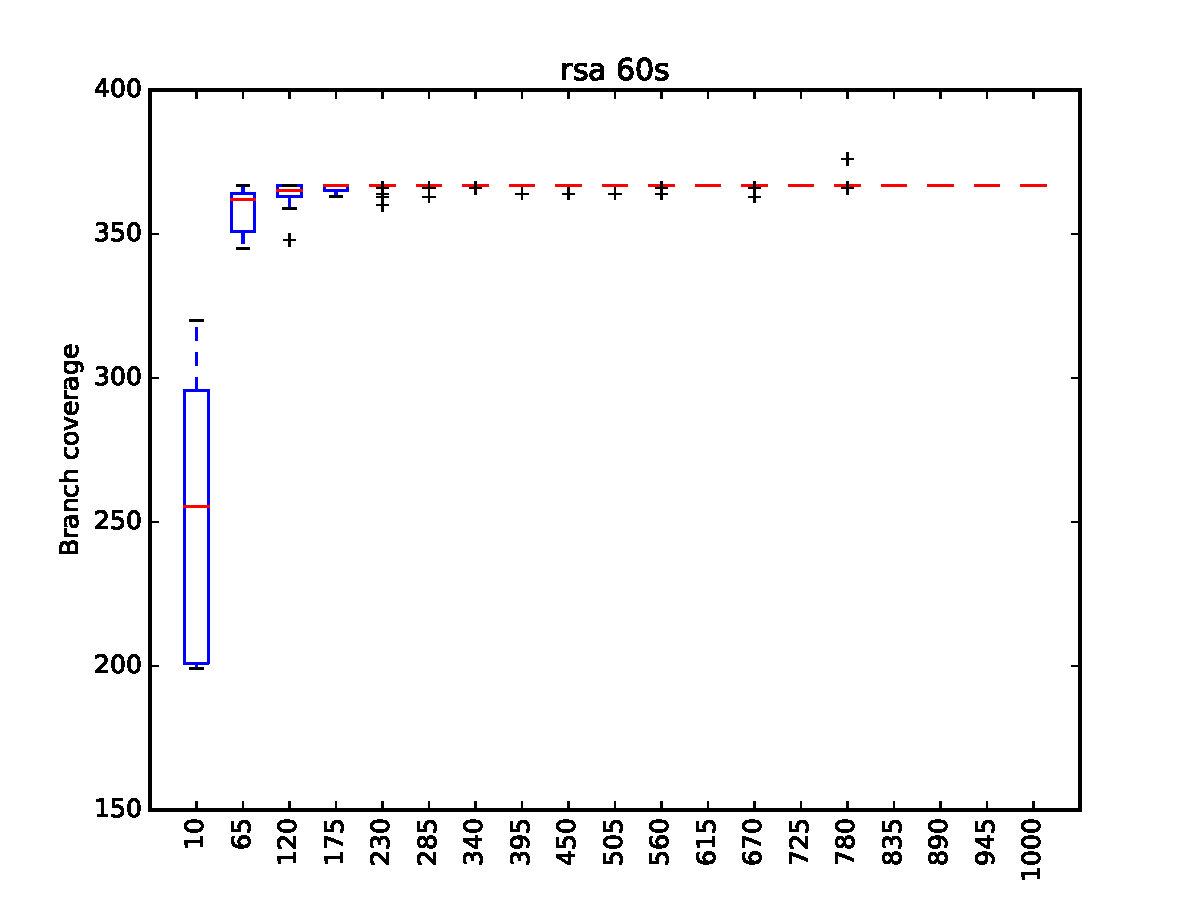
\includegraphics[width=\columnwidth]{graphs/rsarand60}
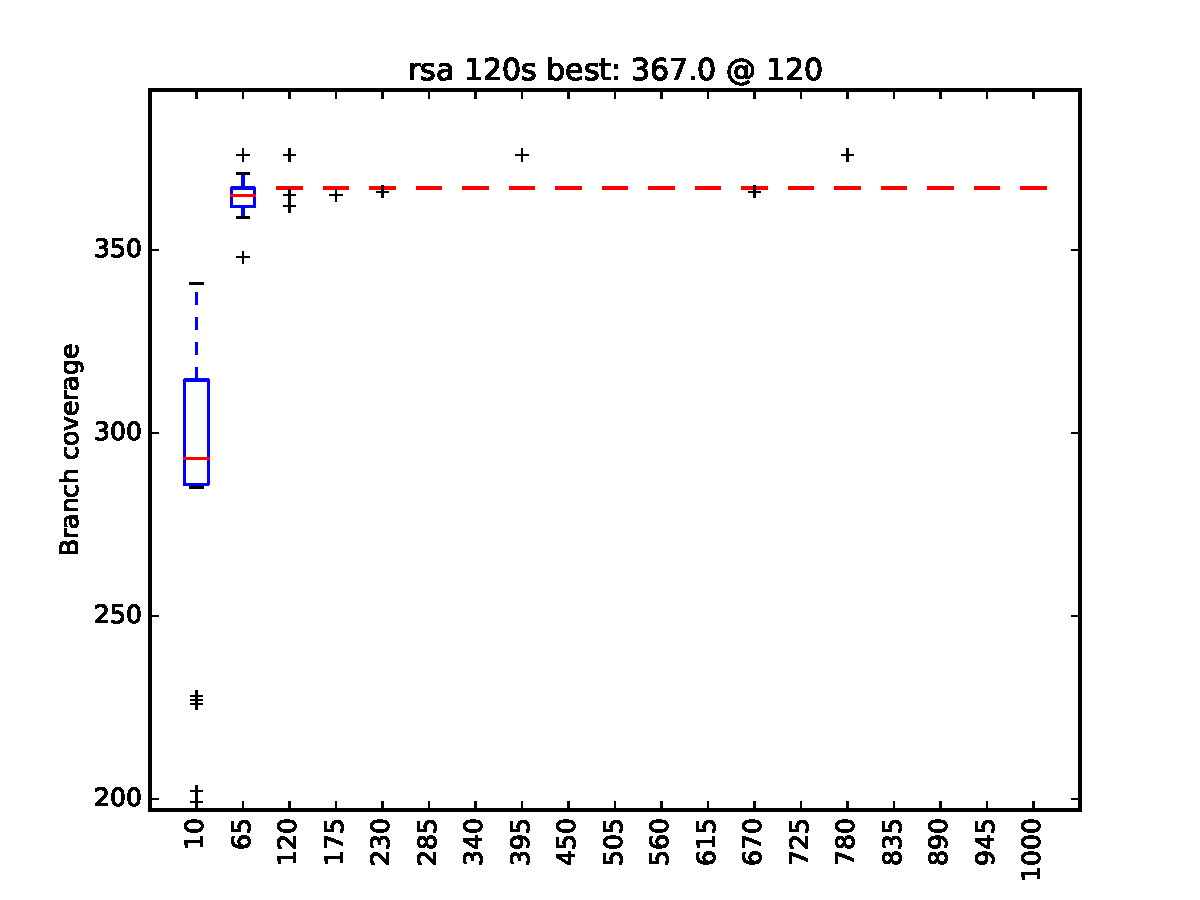
\includegraphics[width=\columnwidth]{graphs/rsarand120}
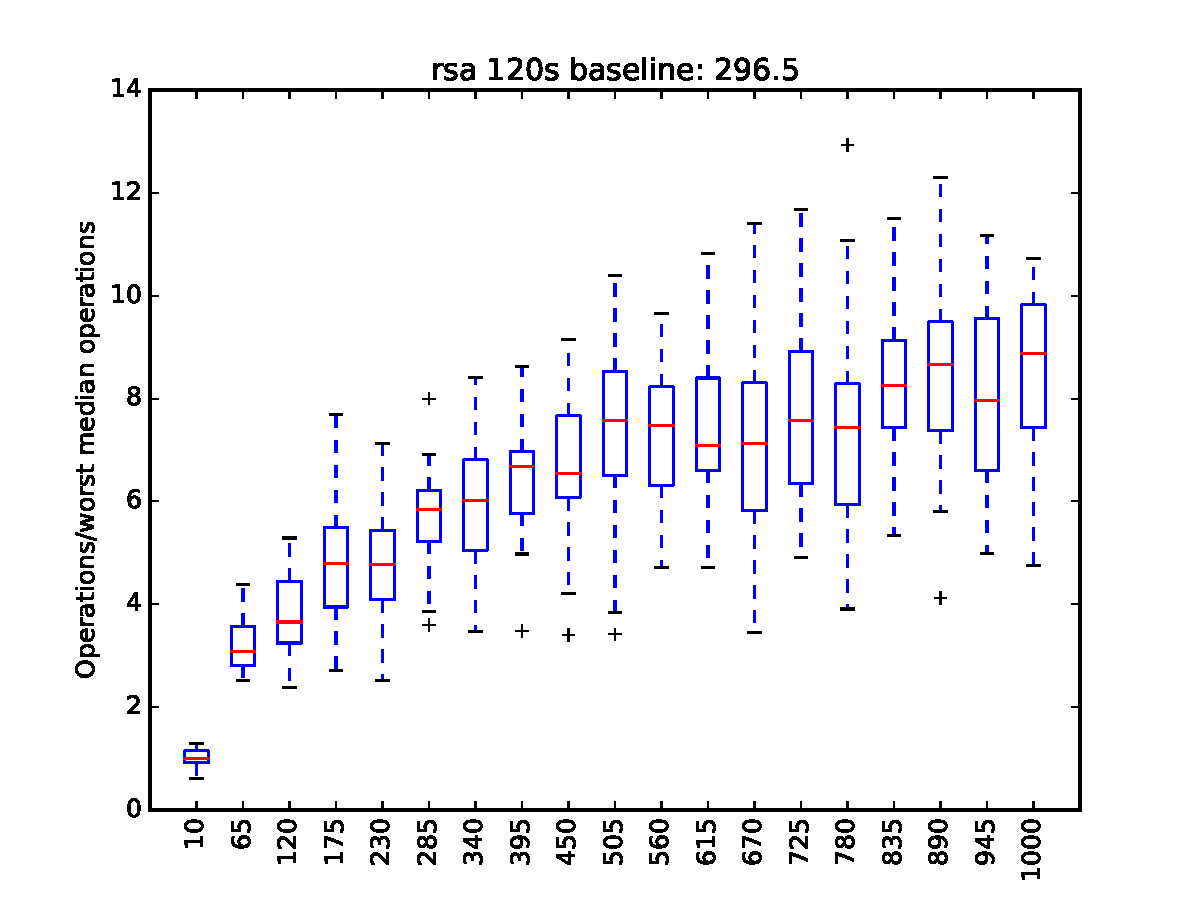
\includegraphics[width=\columnwidth]{graphs/opsrsarand120}
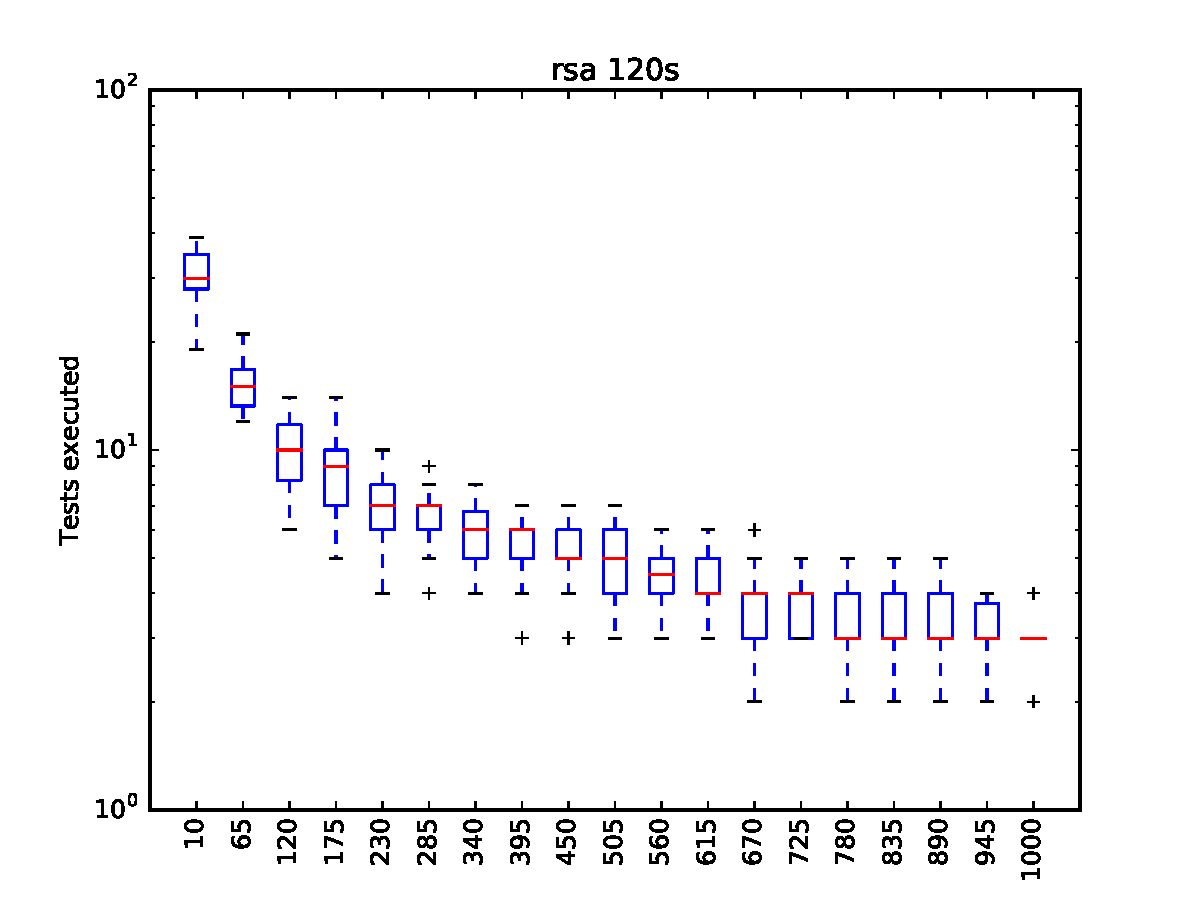
\includegraphics[width=\columnwidth]{graphs/execrsarand120}
\end{figure}


\begin{figure}
%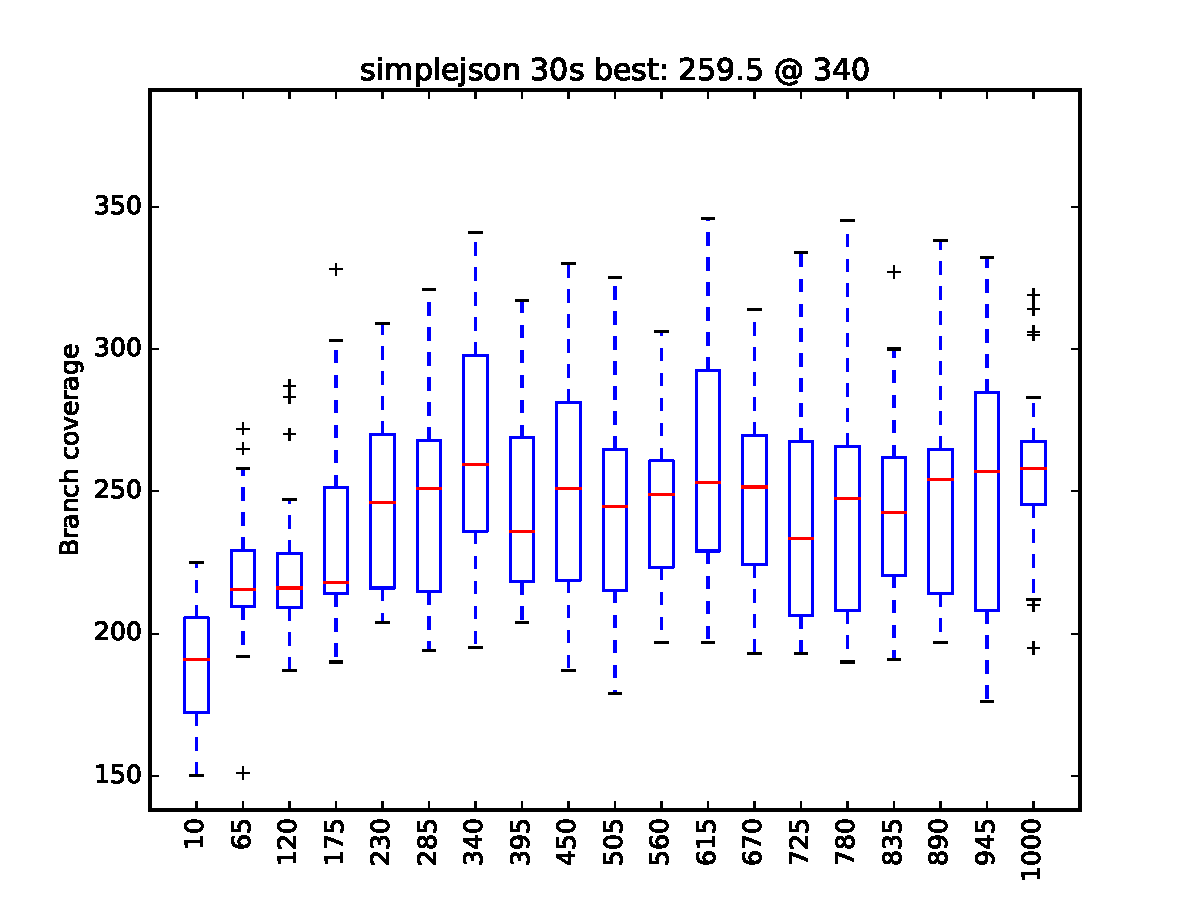
\includegraphics[width=\columnwidth]{graphs/simplejsonrand30}
%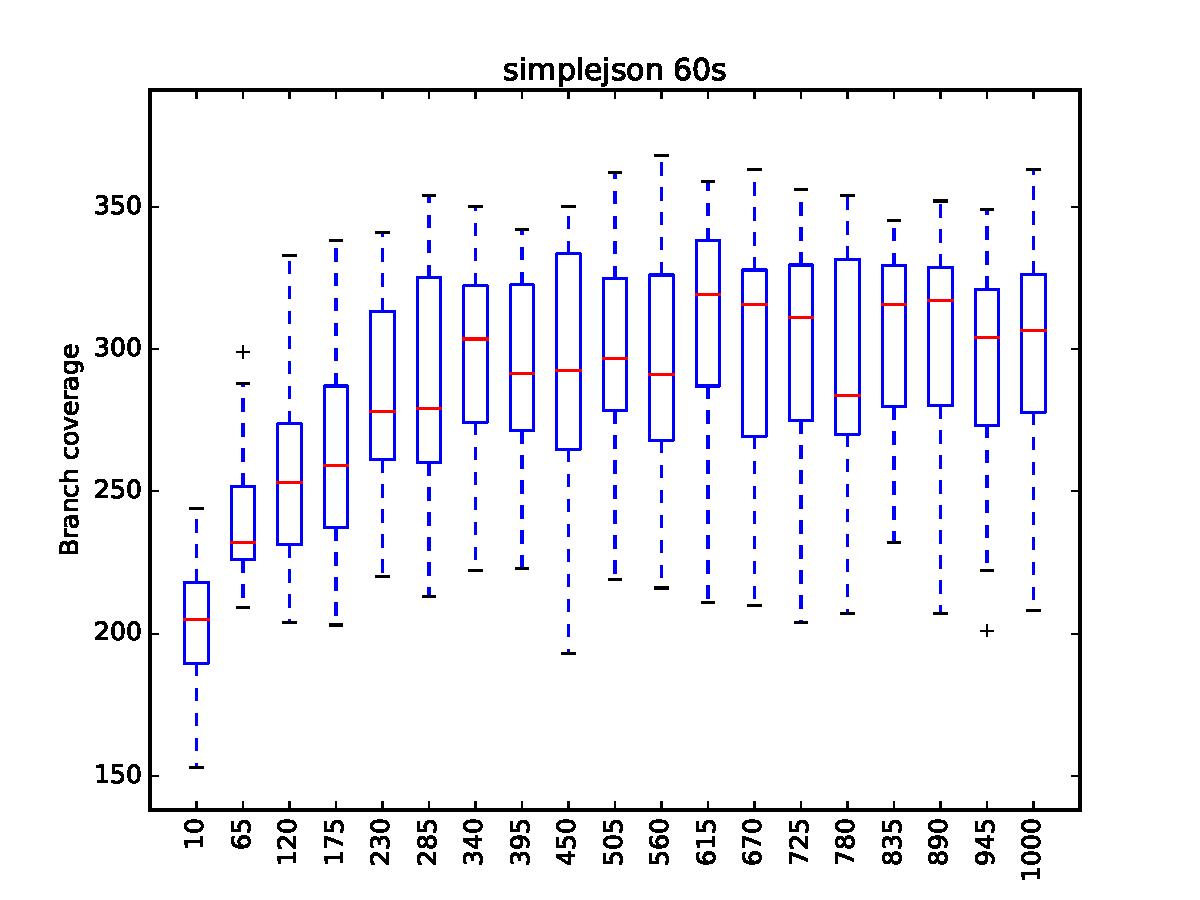
\includegraphics[width=\columnwidth]{graphs/simplejsonrand60}
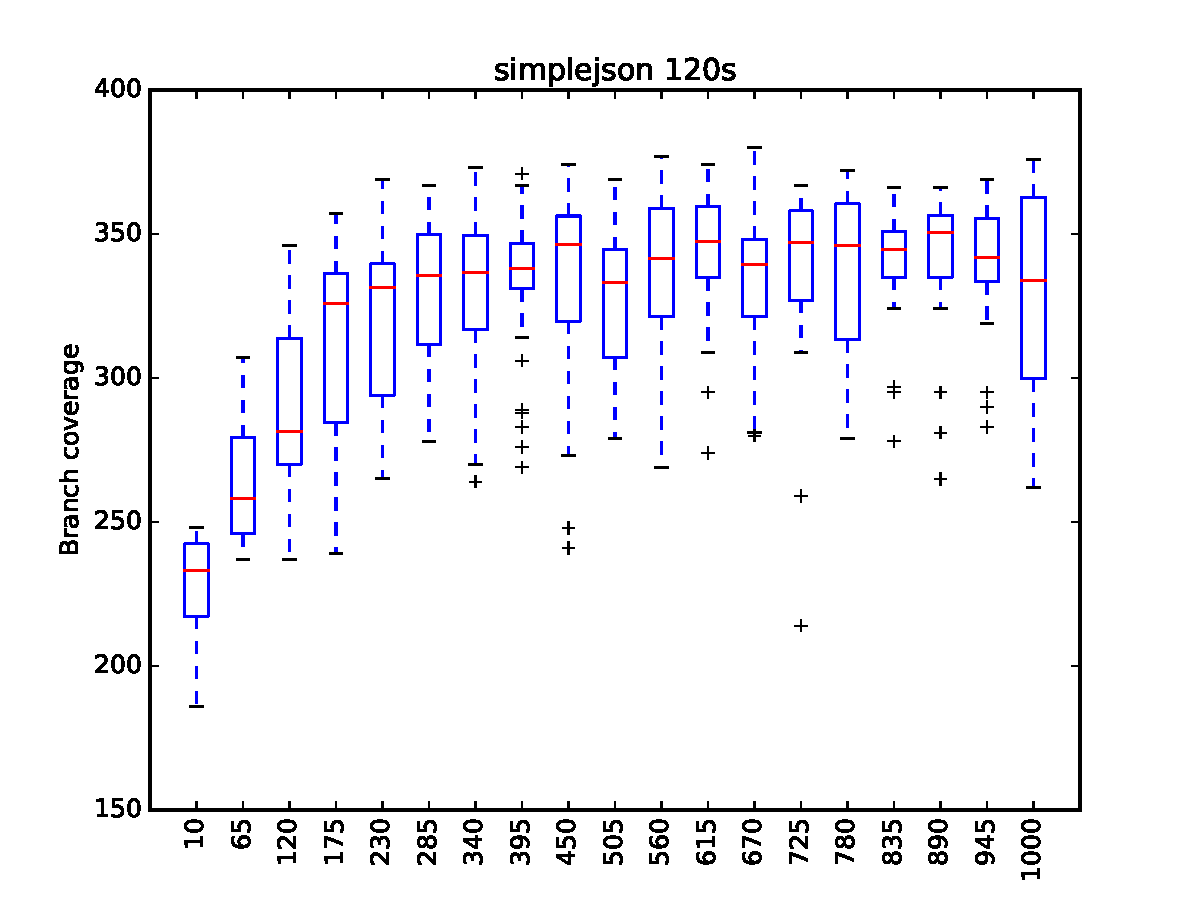
\includegraphics[width=\columnwidth]{graphs/simplejsonrand120}
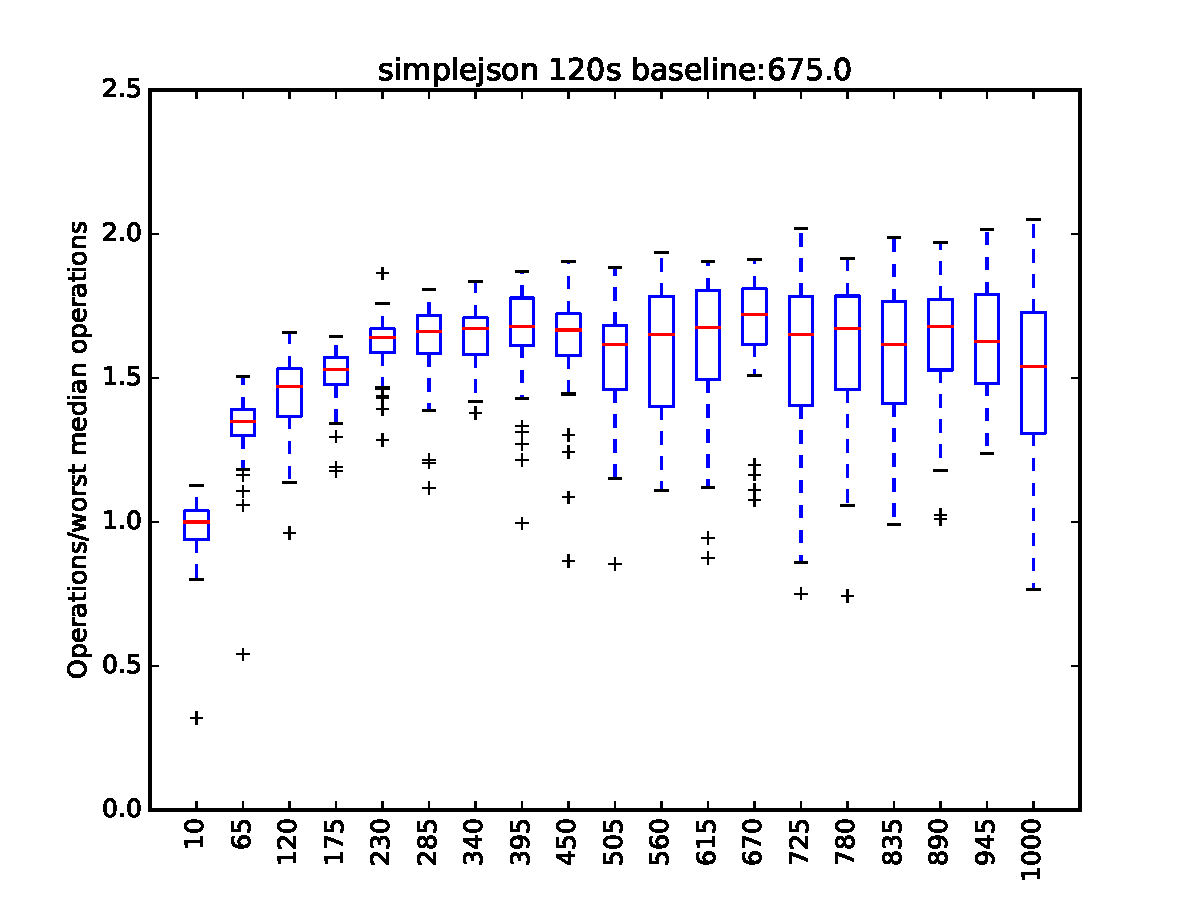
\includegraphics[width=\columnwidth]{graphs/opssimplejsonrand120}
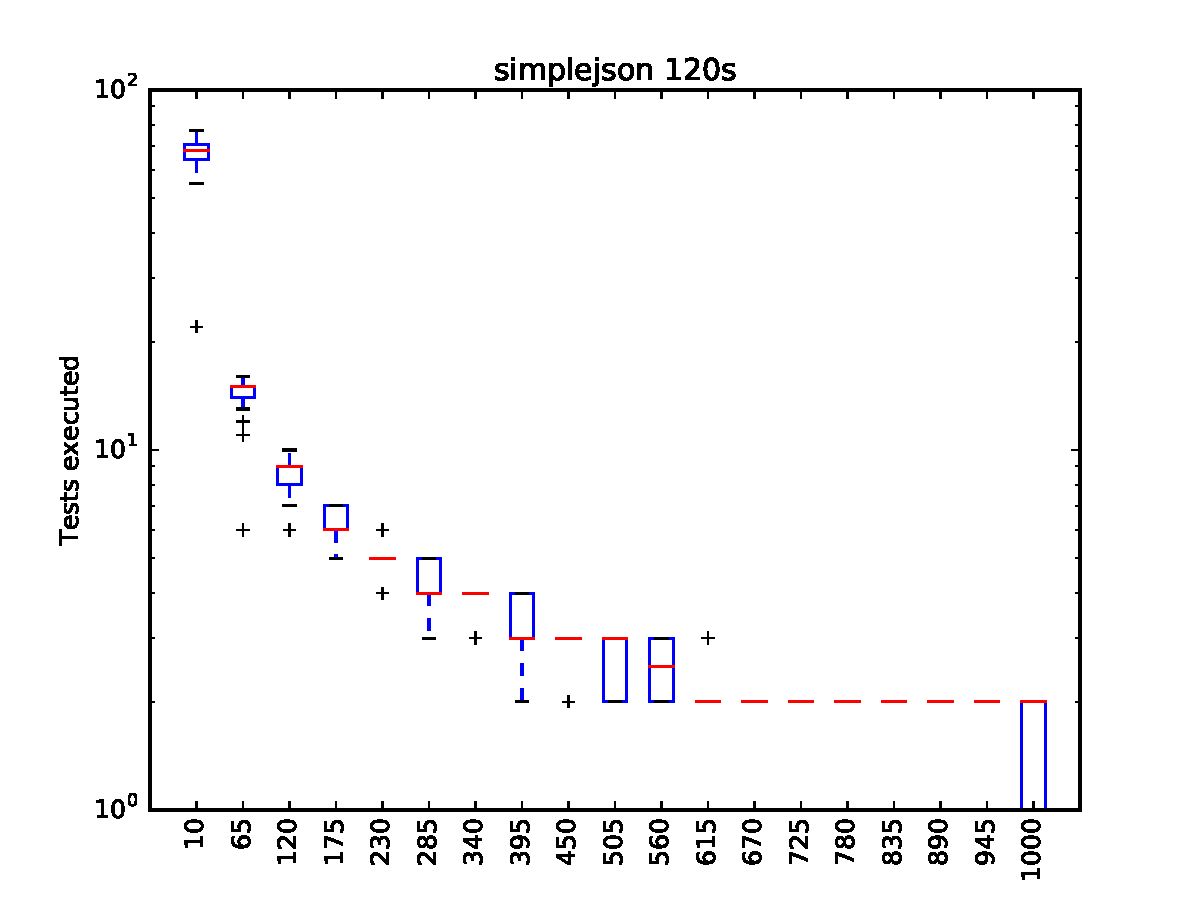
\includegraphics[width=\columnwidth]{graphs/execsimplejsonrand120}
\end{figure}

\begin{figure}
%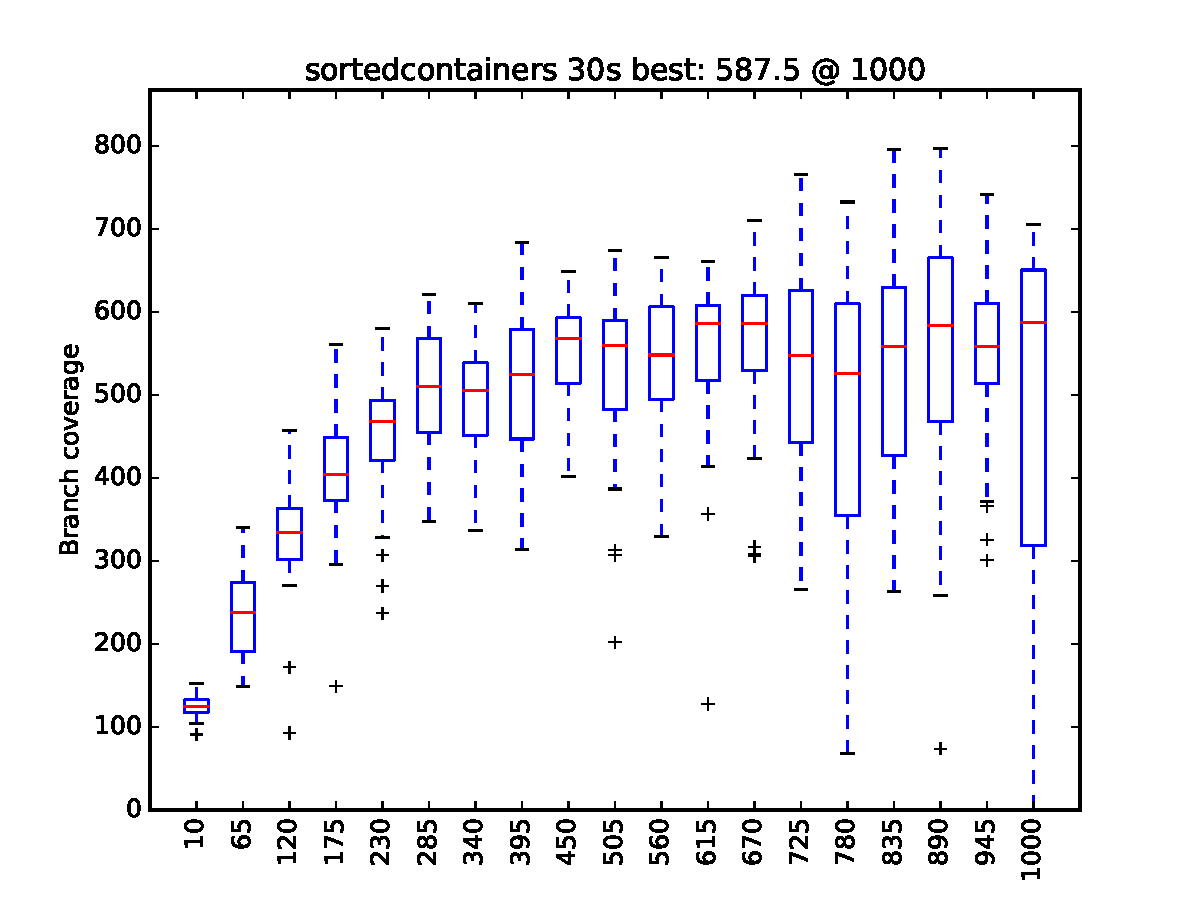
\includegraphics[width=\columnwidth]{graphs/sortedcontainersrand30}
%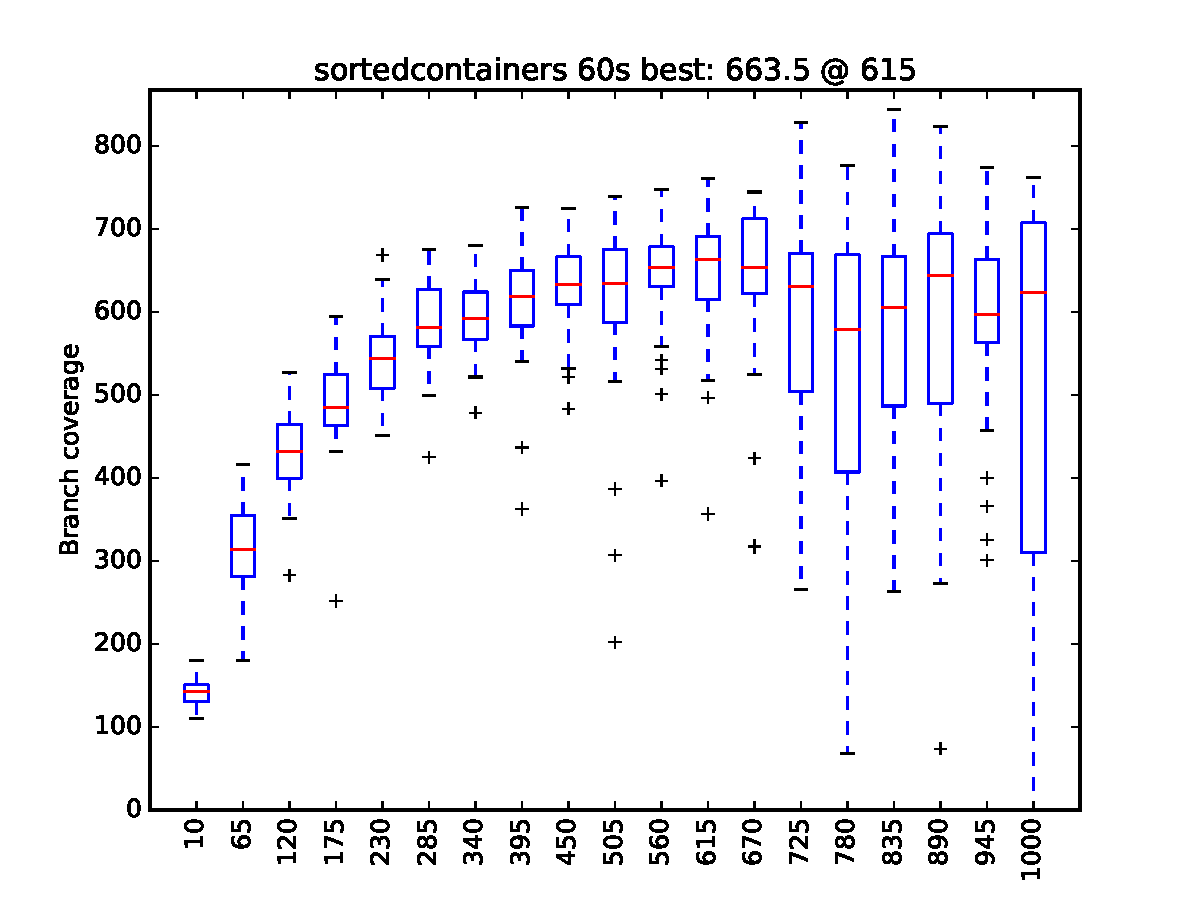
\includegraphics[width=\columnwidth]{graphs/sortedcontainersrand60}
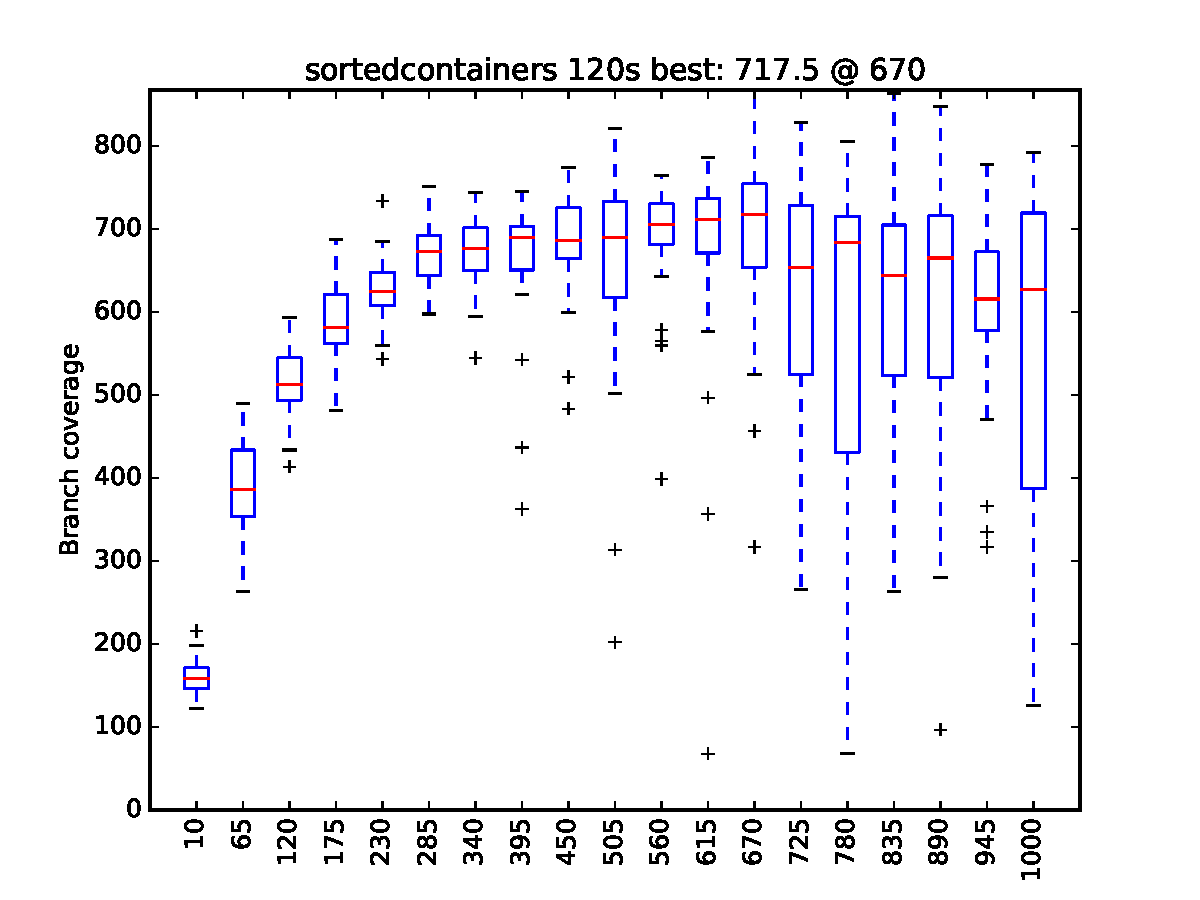
\includegraphics[width=\columnwidth]{graphs/sortedcontainersrand120}
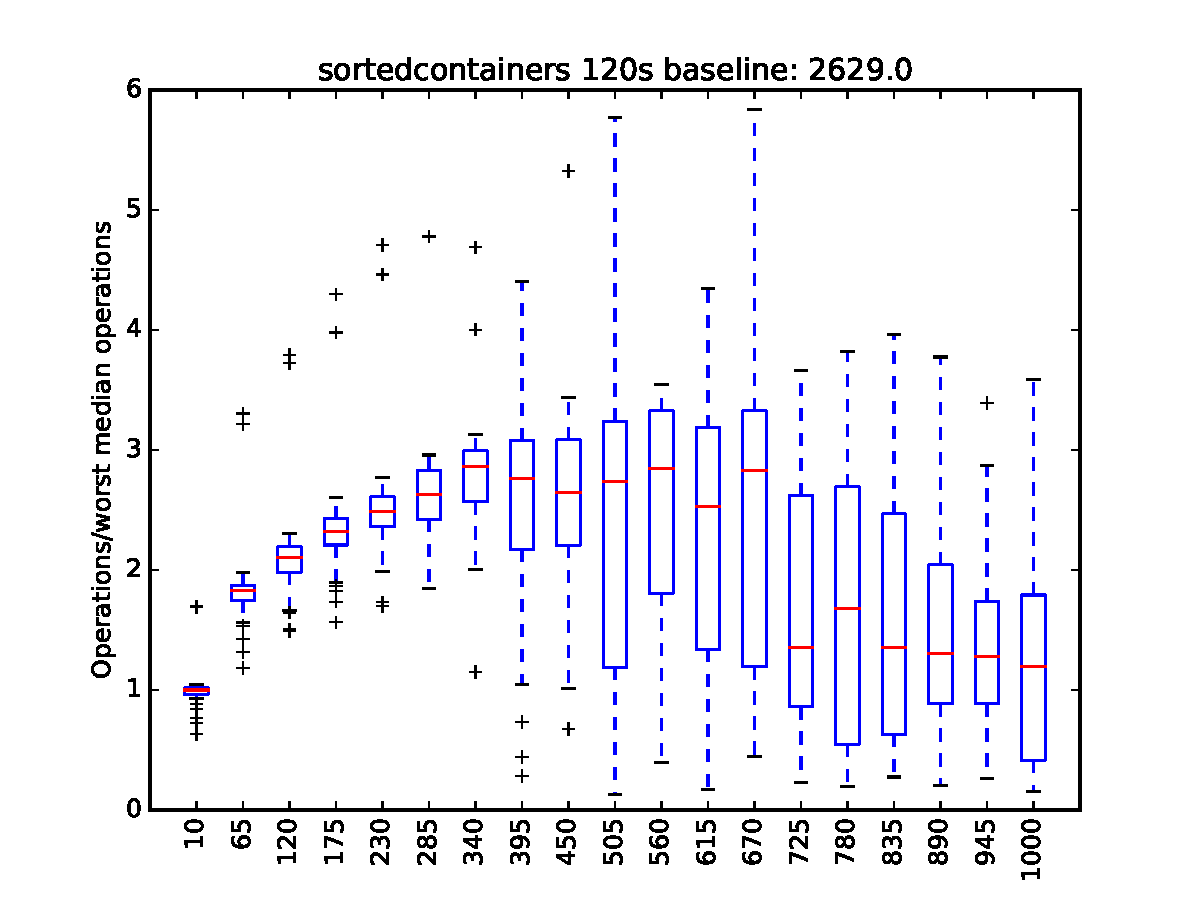
\includegraphics[width=\columnwidth]{graphs/opssortedcontainersrand120}
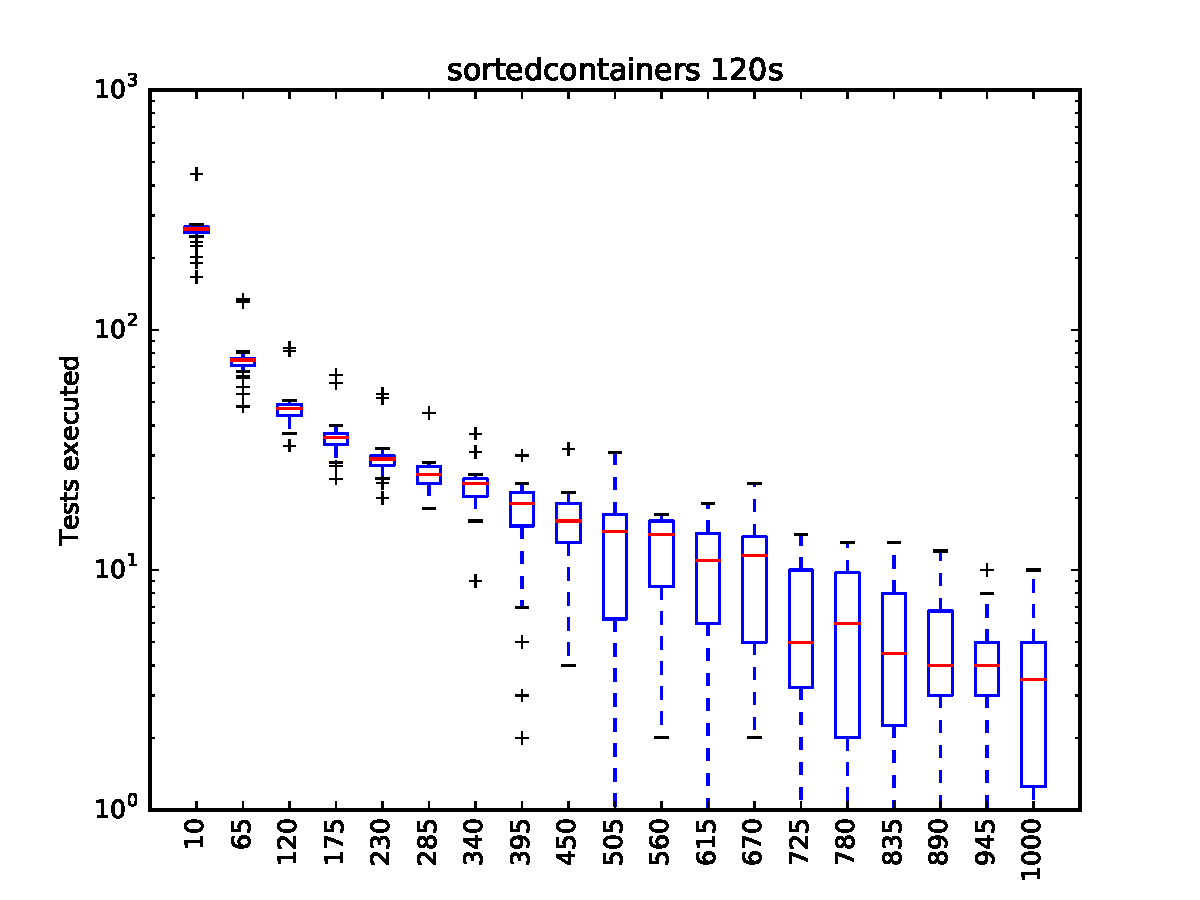
\includegraphics[width=\columnwidth]{graphs/execsortedcontainersrand120}
\end{figure}

\begin{figure}
%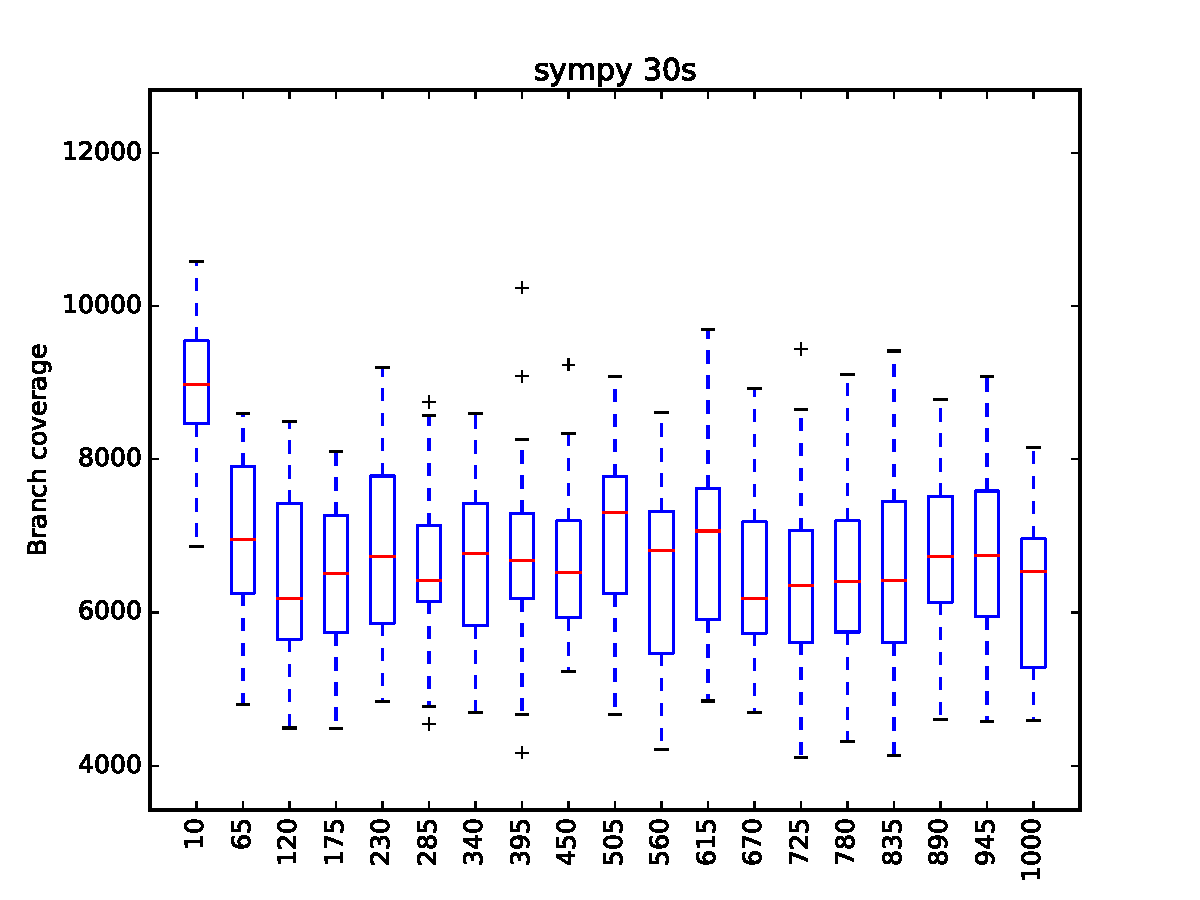
\includegraphics[width=\columnwidth]{graphs/sympyrand30}
%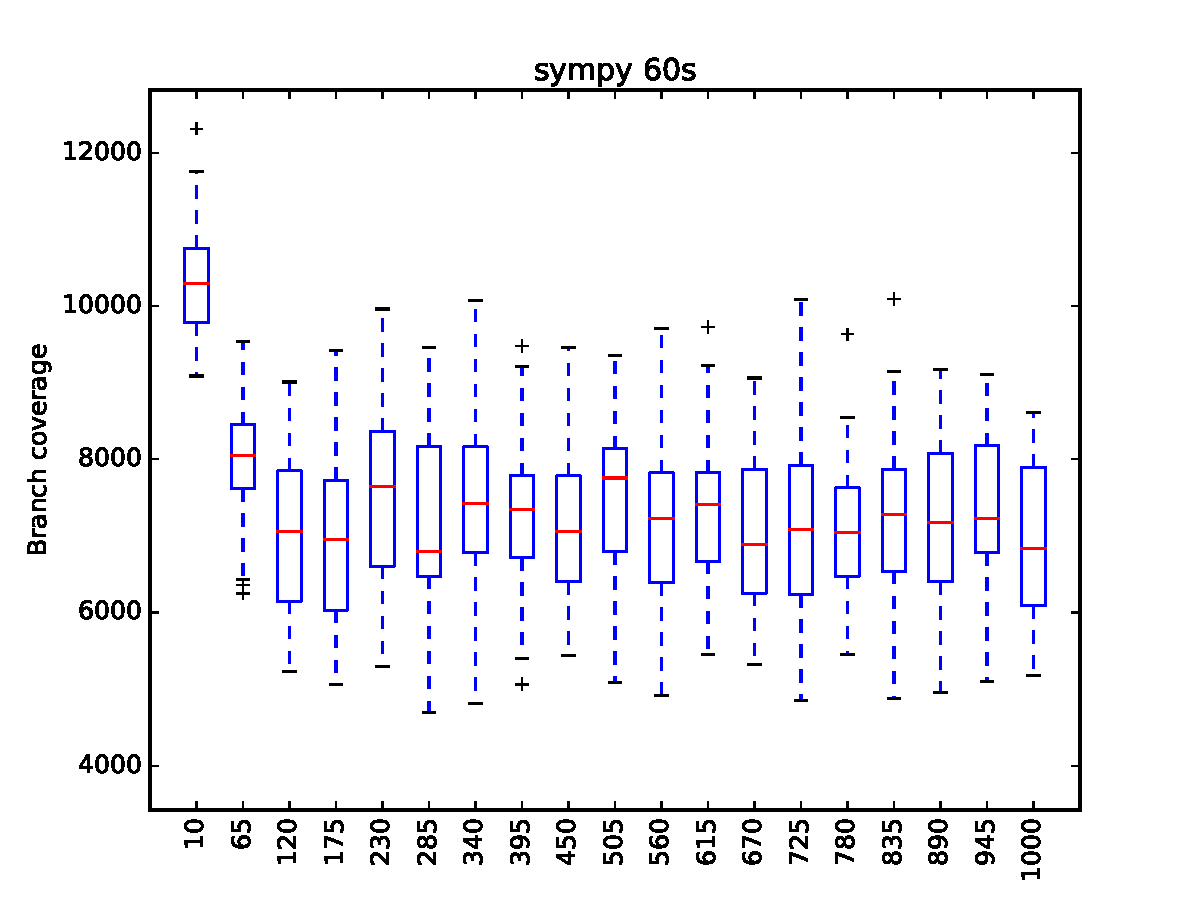
\includegraphics[width=\columnwidth]{graphs/sympyrand60}
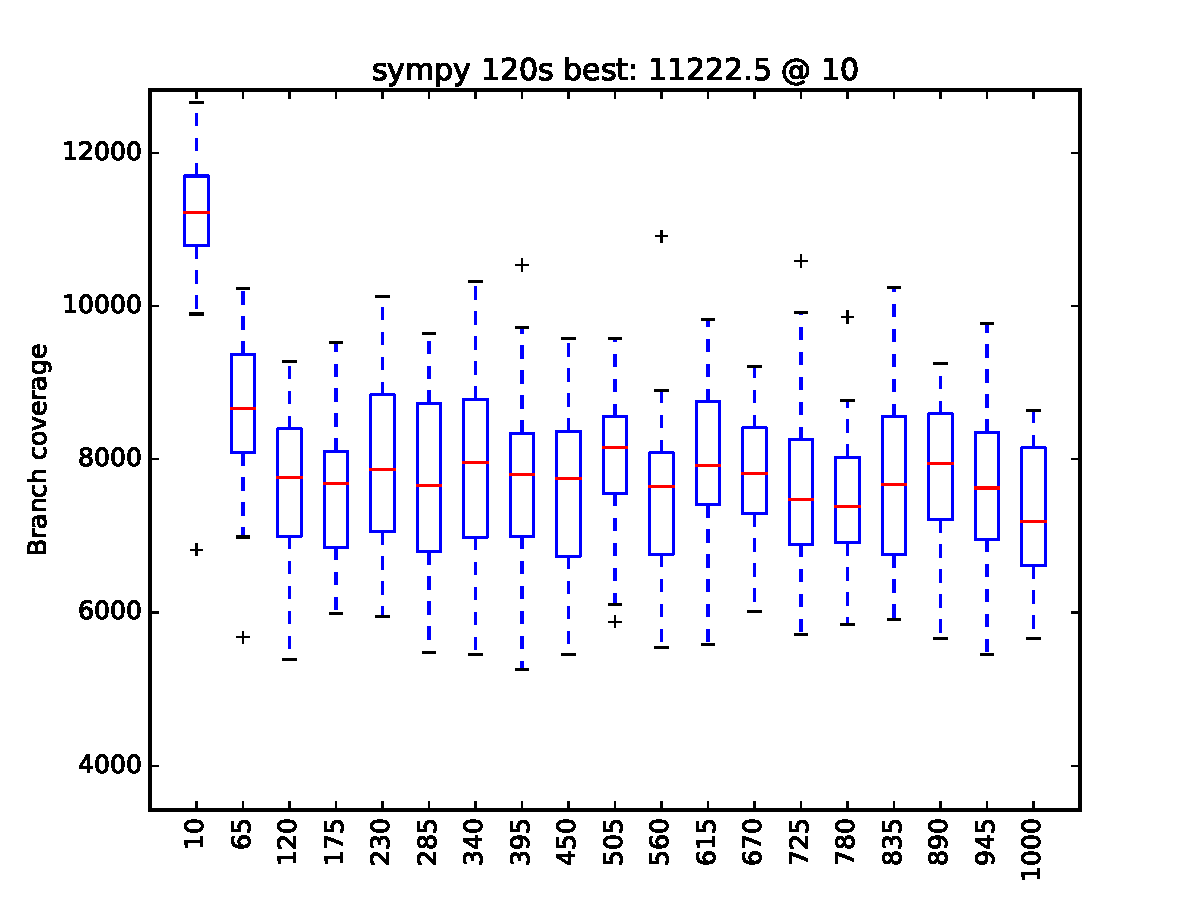
\includegraphics[width=\columnwidth]{graphs/sympyrand120}
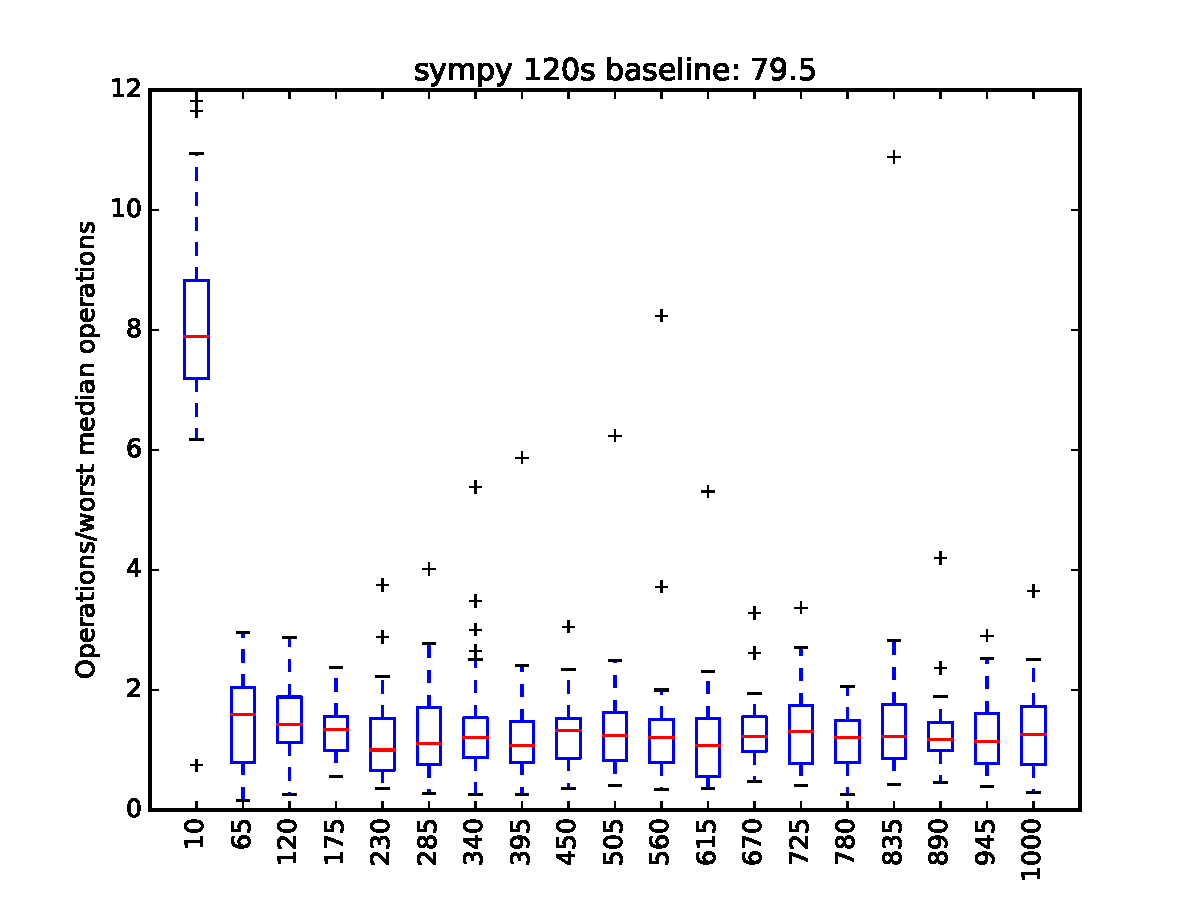
\includegraphics[width=\columnwidth]{graphs/opssympyrand120}
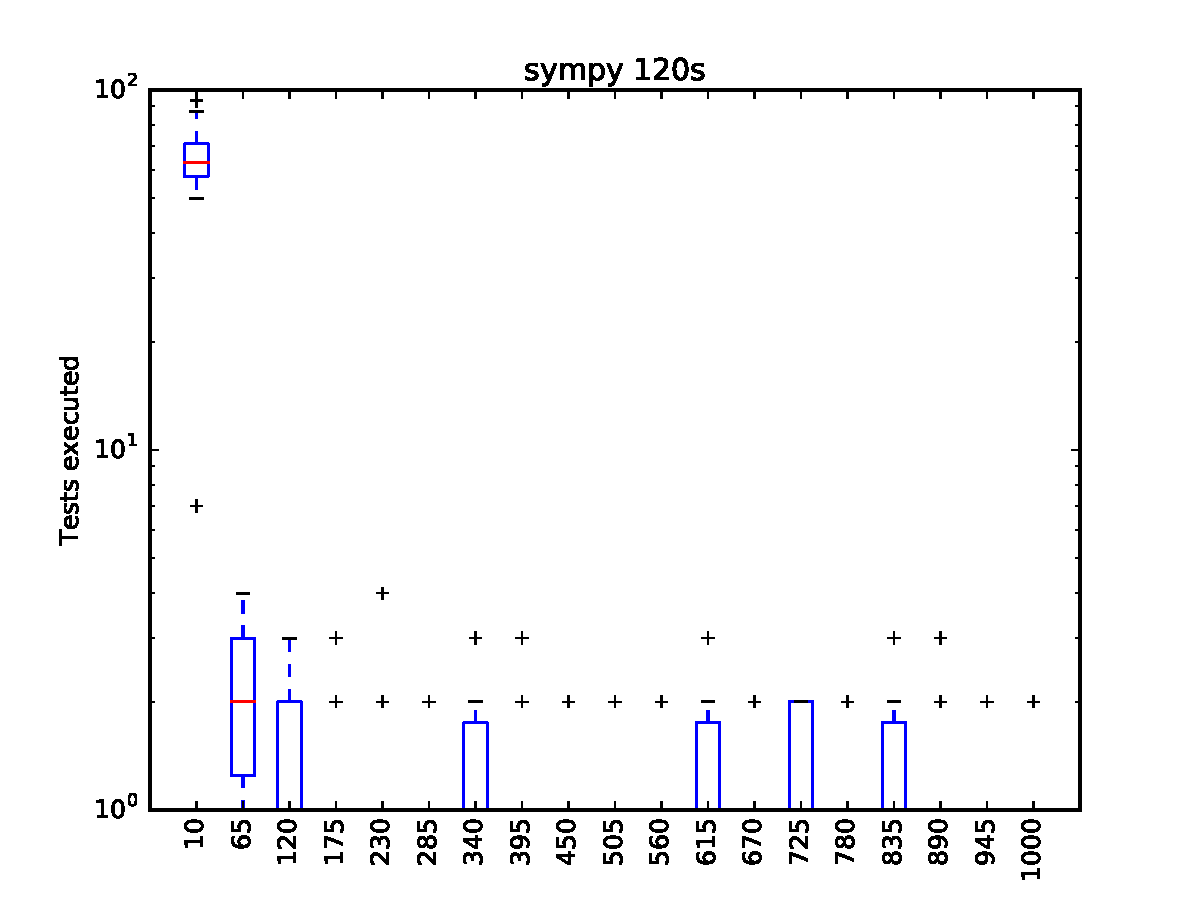
\includegraphics[width=\columnwidth]{graphs/execsympyrand120}
\end{figure}


\begin{figure}
%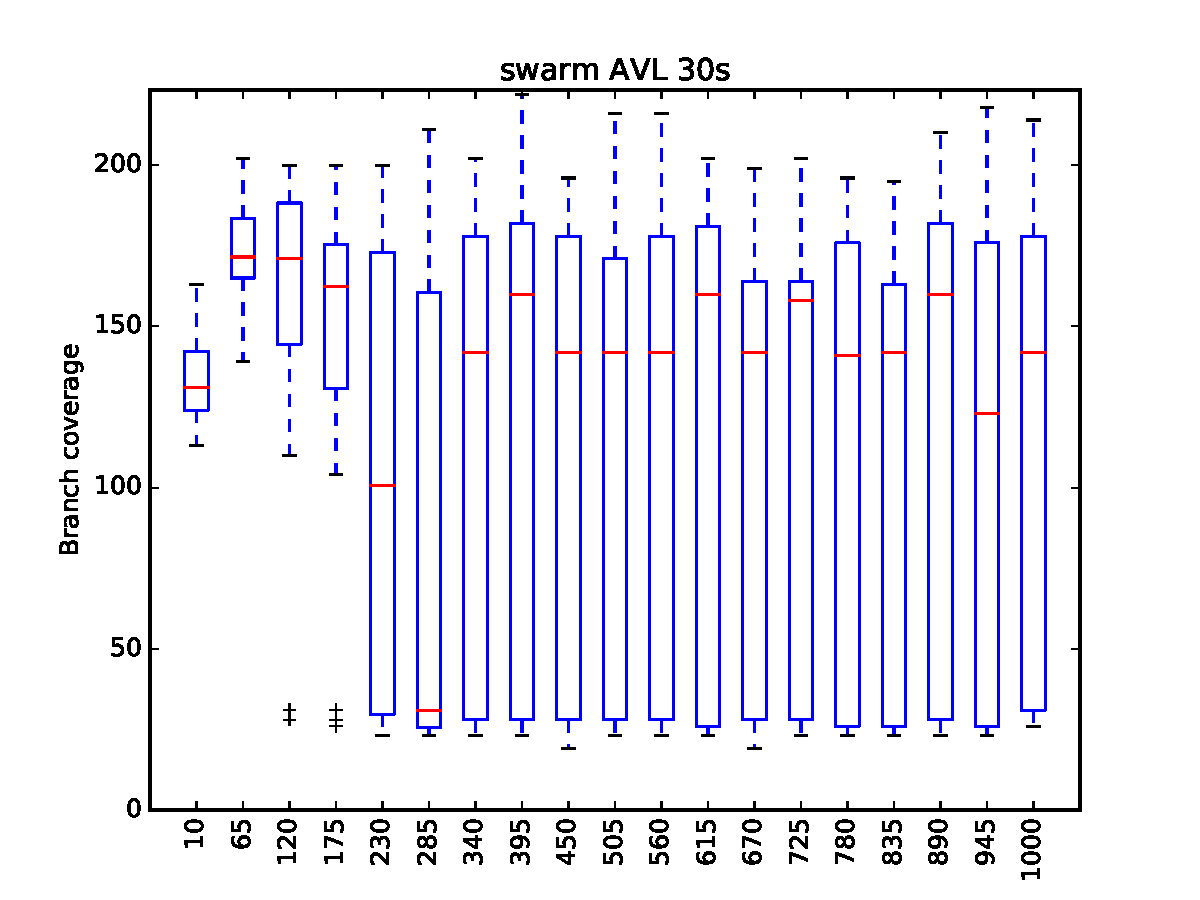
\includegraphics[width=\columnwidth]{graphs/AVLswarm30}
%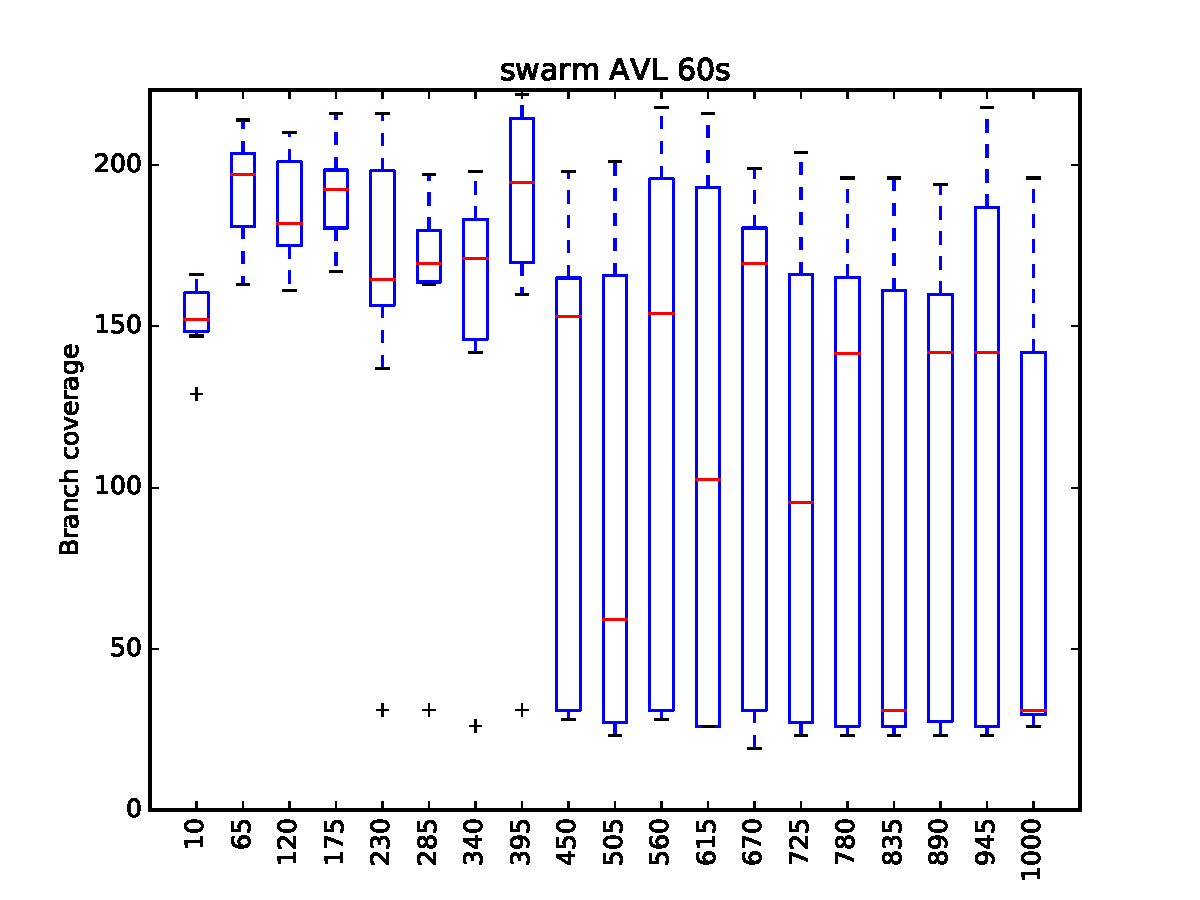
\includegraphics[width=\columnwidth]{graphs/AVLswarm60}
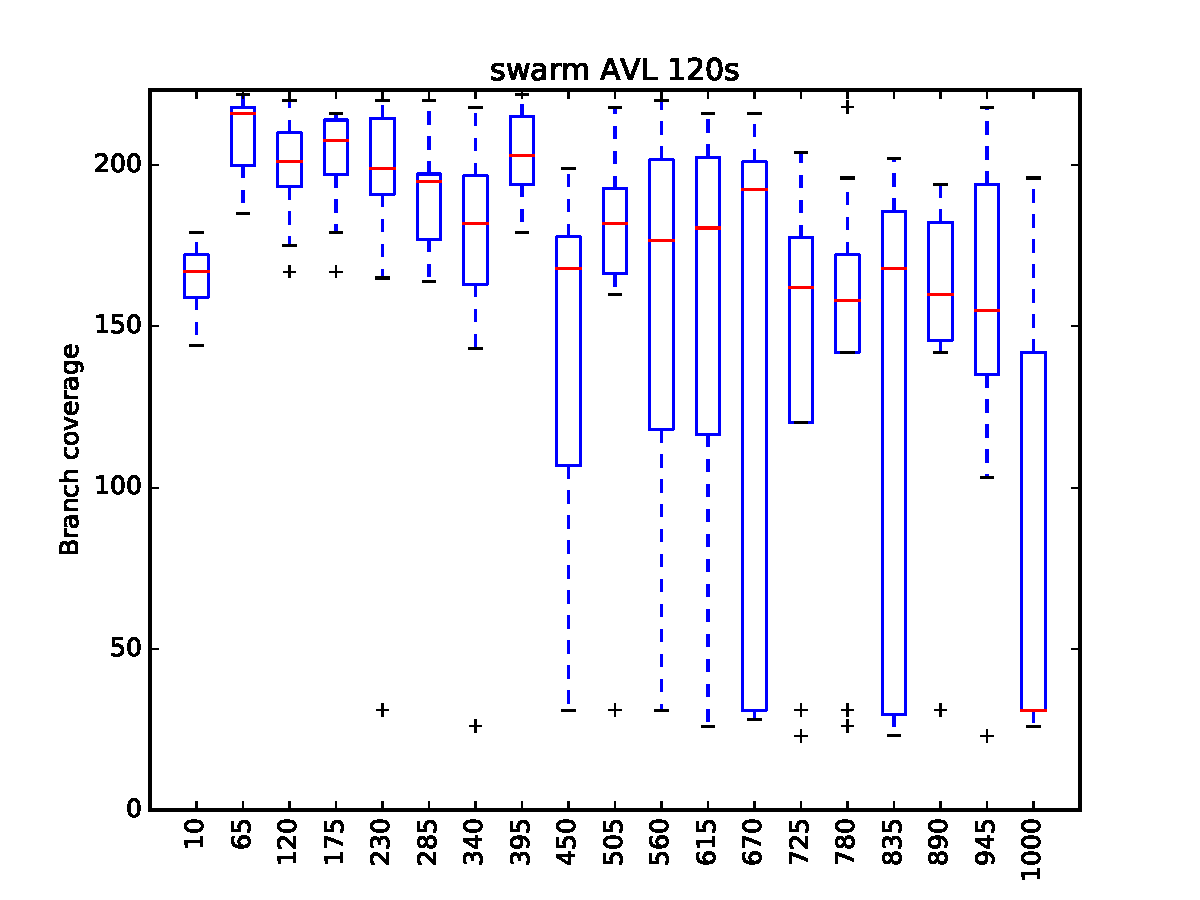
\includegraphics[width=\columnwidth]{graphs/AVLswarm120}
\includegraphics[width=\columnwidth]{graphs/opsavlswarm120}
\includegraphics[width=\columnwidth]{graphs/execavlswarm120}
\end{figure}

\begin{figure}
%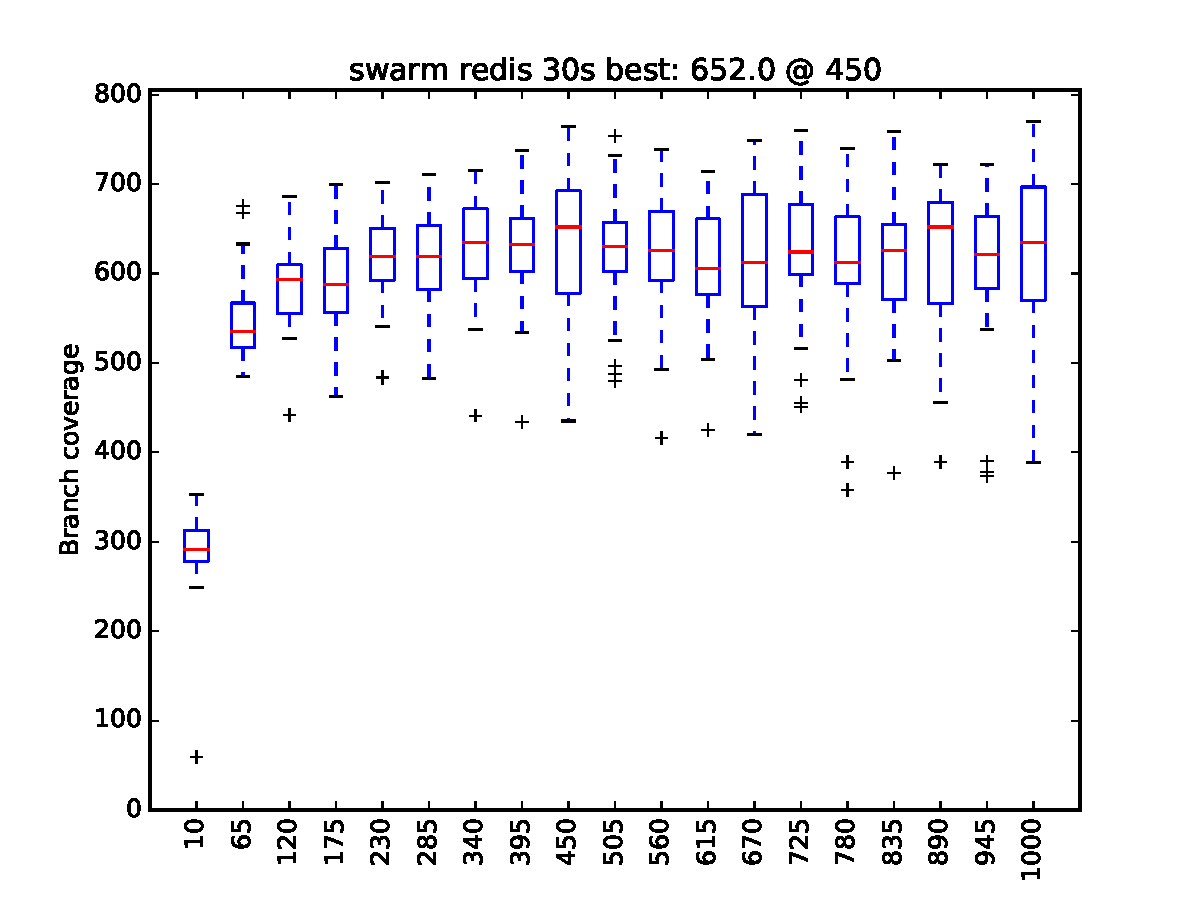
\includegraphics[width=\columnwidth]{graphs/redisswarm30}
%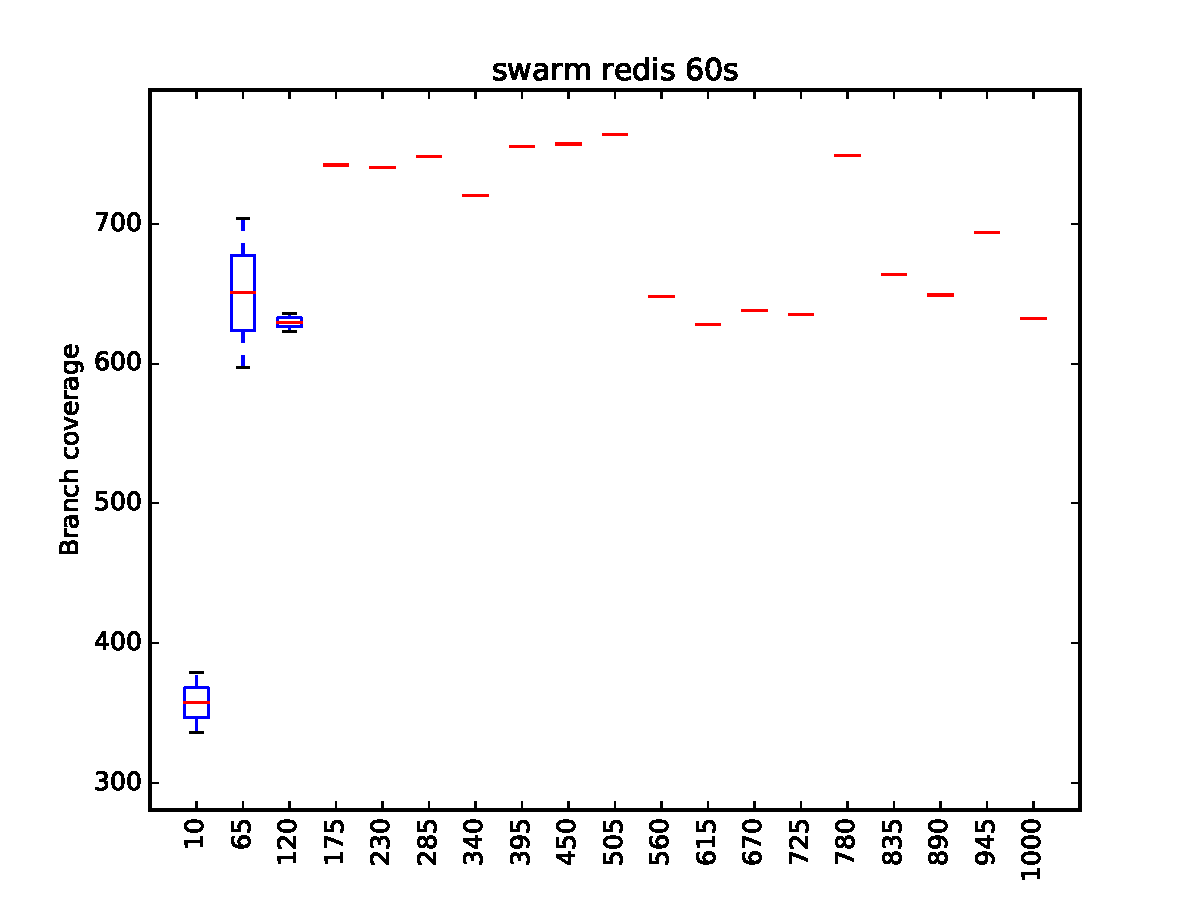
\includegraphics[width=\columnwidth]{graphs/redisswarm60}
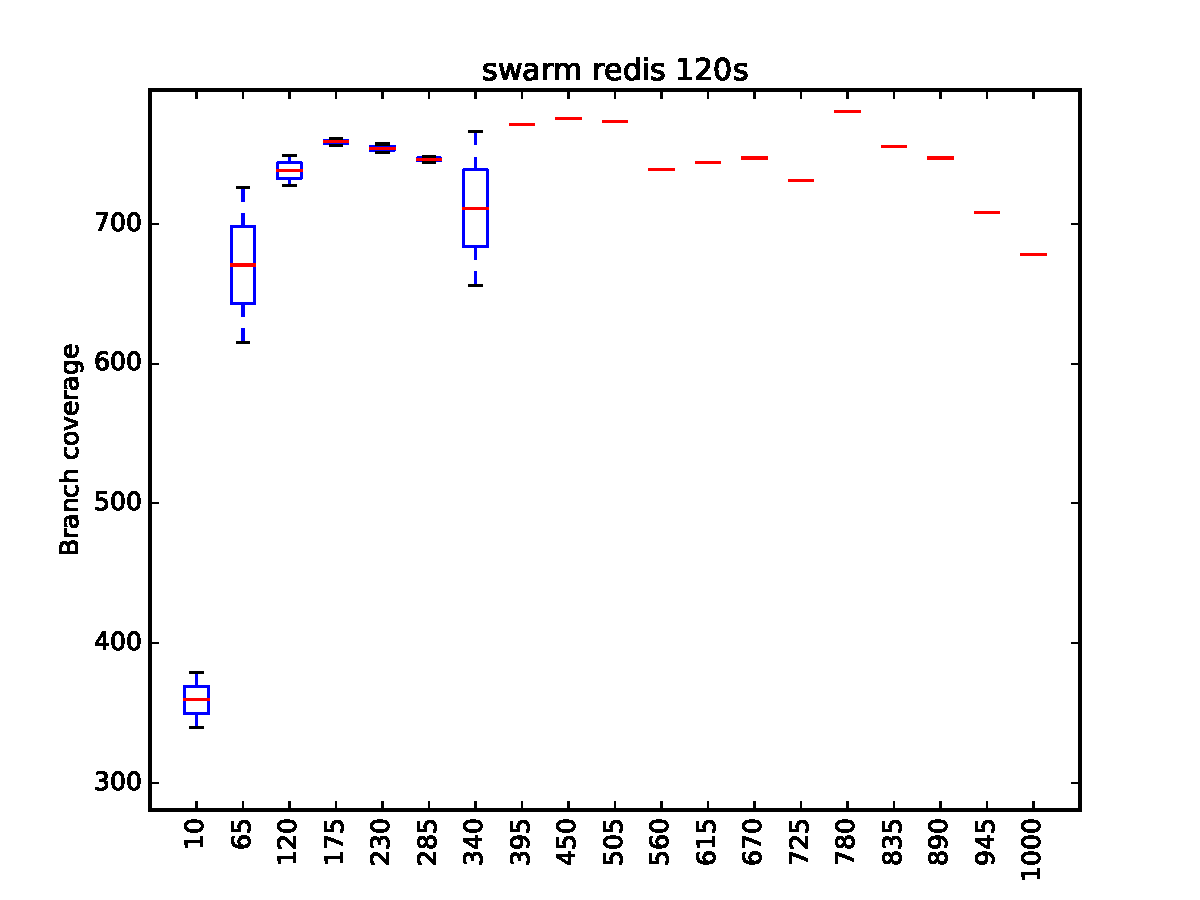
\includegraphics[width=\columnwidth]{graphs/redisswarm120}
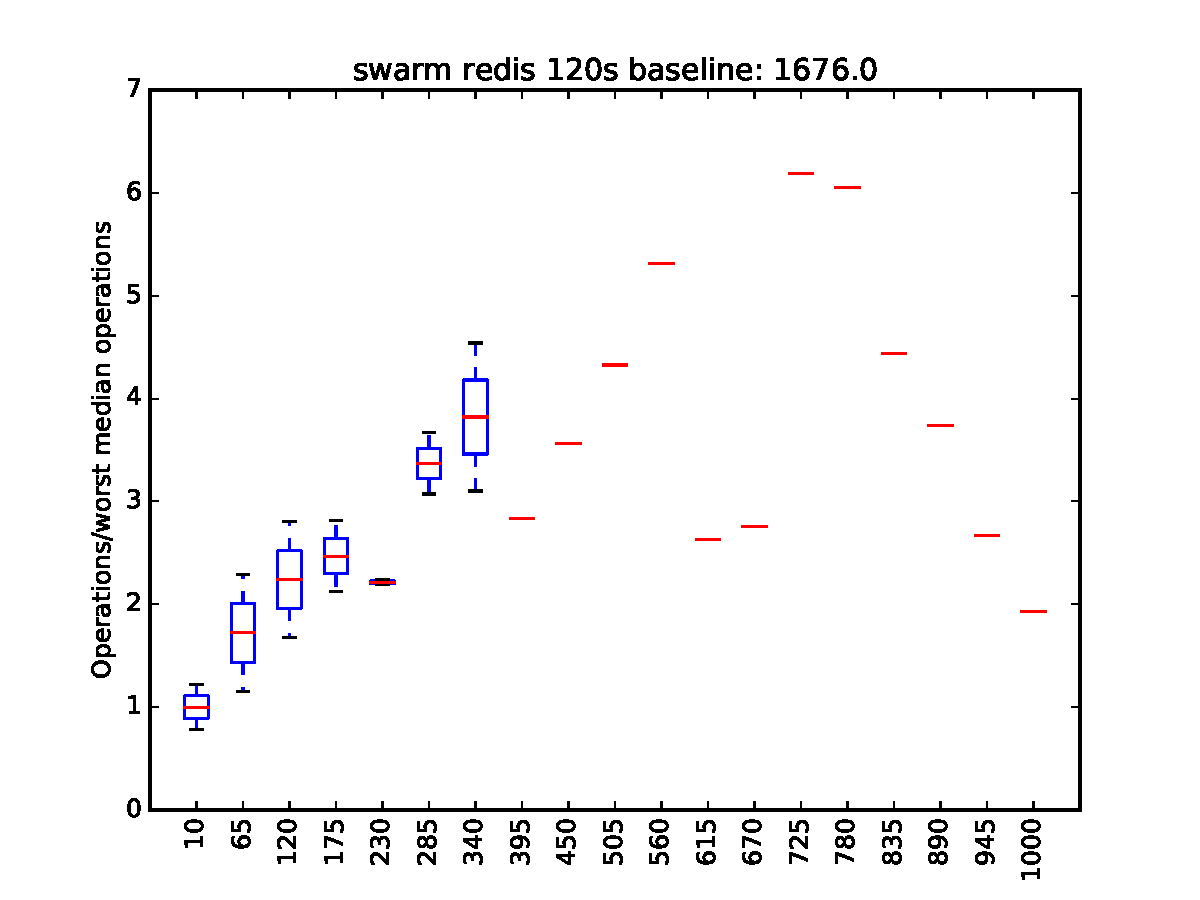
\includegraphics[width=\columnwidth]{graphs/opsredisswarm120}
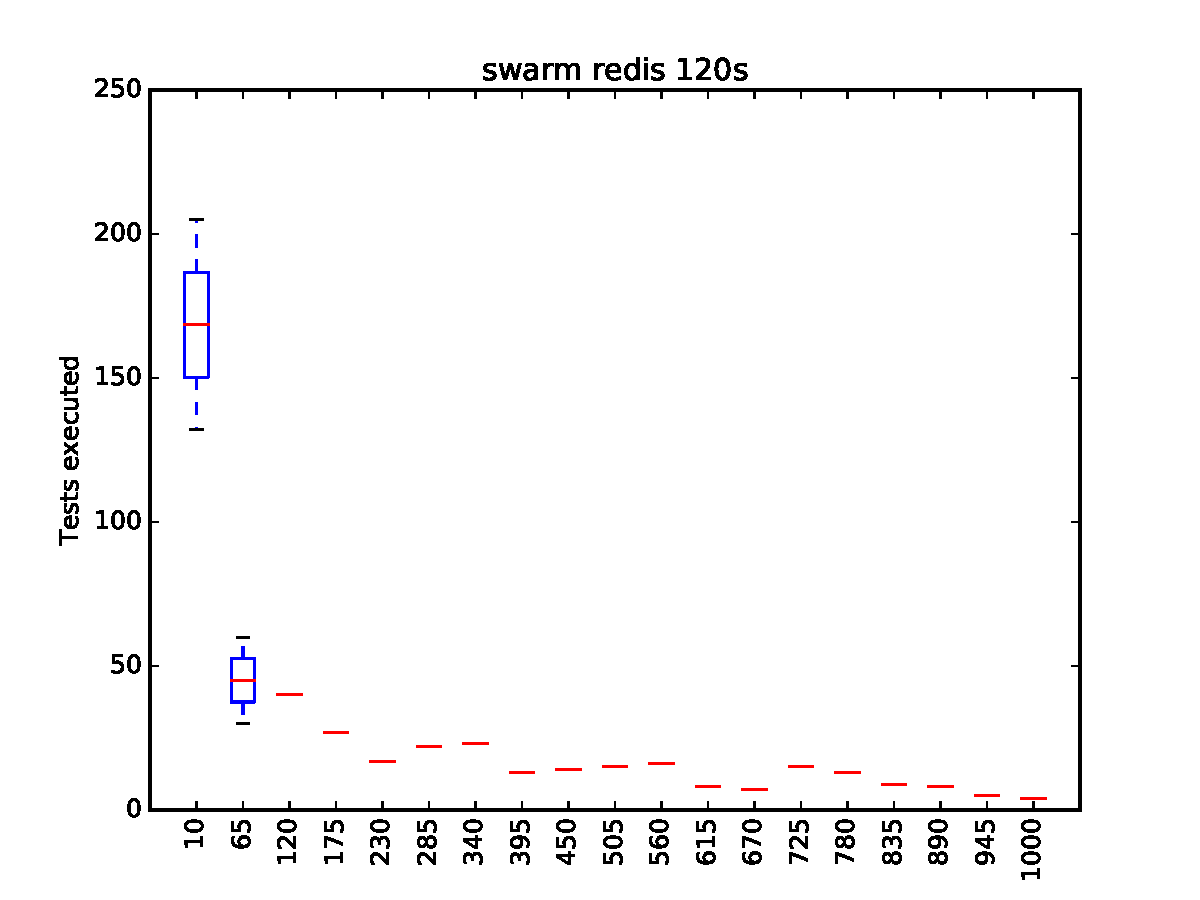
\includegraphics[width=\columnwidth]{graphs/execredisswarm120}
\end{figure}

\begin{figure}
%\includegraphics[width=\columnwidth]{graphs/rsaswarm30}
%\includegraphics[width=\columnwidth]{graphs/rsaswarm60}
\includegraphics[width=\columnwidth]{graphs/rsaswarm120}
\includegraphics[width=\columnwidth]{graphs/opsrsaswarm120}
\includegraphics[width=\columnwidth]{graphs/execrsaswarm120}
\end{figure}


\begin{figure}
%\includegraphics[width=\columnwidth]{graphs/sortedcontainersswarm30}
%\includegraphics[width=\columnwidth]{graphs/sortedcontainersswarm60}
\includegraphics[width=\columnwidth]{graphs/sortedcontainersswarm120}
\includegraphics[width=\columnwidth]{graphs/opssortedcontainersswarm120}
\includegraphics[width=\columnwidth]{graphs/execsortedcontainersswarm120}
\end{figure}

\begin{figure}
%\includegraphics[width=\columnwidth]{graphs/sympyswarm30}
%\includegraphics[width=\columnwidth]{graphs/sympyswarm60}
\includegraphics[width=\columnwidth]{graphs/sympyswarm120}
\includegraphics[width=\columnwidth]{graphs/opssympyswarm120}
\includegraphics[width=\columnwidth]{graphs/execsympyswarm120}
\end{figure}